\title{LAC - Assignment 5}

\documentclass[11pt]{article}
\usepackage[utf8]{inputenc}
\usepackage[english]{babel}
%\documentclass[11pt]{article}
\usepackage{setspace} %to set line spacing
\usepackage{fullpage} %uses up more of the page
\usepackage{titlesec} %to edit section titles
\usepackage{graphicx} %to import graphics
%\usepackage{siunitx}
%\usepackage{pdflscape}
%\usepackage{longtable}
\usepackage[title]{appendix}
\usepackage{float}%for the H option in figures
\usepackage{bigstrut} %for excel to latex tabular converter
\usepackage{lscape} %for landscape pages
\usepackage{pdfpages}
\usepackage{amsmath} %\begin{align} - \end{align}
\usepackage[framed,numbered]{mcode}  %imports and formats .m files
\usepackage{multirow}
%\usepackage{tikz}
%\usetikzlibrary{shapes.geometric, arrows}
%\usepackage{iftex}
%\usepackage{array,booktabs}
\usepackage{subcaption}
\usepackage{bm} %Bold in mathmode
%\usepackage{chngcntr}
%\counterwithout{figure}{section}
%\counterwithout{table}{section}
%\counterwithout{figure}{chapter}
%\counterwithout{table}{chapter}
\captionsetup{font=small}
%\usepackage[labelfont=bf]{caption}
%\newcolumntype{C}[1]{>{\centering\arraybackslash}m{#1}}

% BIBLIOGRAPHY SETTINGS
\usepackage{natbib} %for harvard referencing
\bibliographystyle{abbrvnat}
\setcitestyle{numbers,square}

%\cite{berg2009active}  -> [1]
%\citet{berg2009active}  -> Berg et al. [1]
%\citeauthor{berg2009active} -> Berg et al.




\graphicspath{{./Figures/}}

%\myFigure[figure size]{filename.jpg}{Description}{figx}
%\myFigure[]{}{}{}
\newcommand{\myFigure}[4][0.8]{
\begin{figure}[H] 

	\centering
	\setlength\fboxsep{1pt}
	\setlength\fboxrule{0.5pt}

	\includegraphics[width=#1\textwidth]{#2}
	\caption{\small #3}
	\label{#4}
\end{figure}
}

\newcommand{\myFigureSideSide}[8]{
\begin{figure}[H] 

	\centering
    \begin{subfigure}[b]{0.49\textwidth}
    \centering
    \includegraphics[width=1\textwidth]{#1}
    \caption{\small #2}
	\label{#3}
    \end{subfigure}
    \begin{subfigure}[b]{0.49\textwidth}
    \centering
    \includegraphics[width=1\textwidth]{#4}
    \caption{\small #5}
	\label{#6}
    \end{subfigure}   
% 	\setlength\fboxsep{1pt}
% 	\setlength\fboxrule{0.5pt}
	\caption{\small #7}
	\label{#8}
\end{figure}
}



\setlength{\parindent}{0cm} %removes paragraph indentation
%\newcommand{\sr}{\rule[-0.45cm]{0pt}{0.9cm}}


\titleformat{\subsection}{\normalsize\bfseries}{\thesubsection}{1em}{}
\titleformat{\subsubsection}{\normalsize\it\bfseries}{\thesubsubsection}{1em}{}
 \newcommand{\hinfty}{$\mathcal{H}_\infty$~} 
 \newcommand\norm[1]{\left\lVert#1\right\rVert}

\begin{document}

\includepdf{CoverPage}
%\begin{titlepage}

\includepdf{CoverPage}
\newcommand{\HRule}{\rule{\linewidth}{0.5mm}} % Defines a new command for the horizontal lines, change thickness here

\center % Center everything on the page

%----------------------------------------------------------------------------------------
%	HEADING SECTIONS
%----------------------------------------------------------------------------------------
\begin{figure}[H]
\centering

\includegraphics[width=40mm]{Figures/DTU_Logo.png}
\end{figure}
\vspace{3cm}
% \textsc{\LARGE TU Delft}\\[1.5cm] % Name of your university/college
\textsc{\Large Active Tip Deflection Control For Wind Turbines}\\[0.5cm] 

%----------------------------------------------------------------------------------------
%	TITLE SECTION
%----------------------------------------------------------------------------------------

\HRule \\[0.4cm]
\setstretch{1.3}
{ \huge \bfseries Literature Review}\\[0.4cm] % Title of your document
\setstretch{1}
\HRule \\[1.5cm]


%----------------------------------------------------------------------------------------
%	AUTHOR SECTION
%----------------------------------------------------------------------------------------

\begin{center}
\begin{tabular}{rll}
&\\
\large
Jaime Liew && s141777 \\

\end{tabular}
\end{center}

\vspace{3cm}
~
~

\vspace{2cm}

% If you don't want a supervisor, uncomment the two lines below and remove the section above
%\Large \emph{Supervisor:}\\
%\textcolor{red}{John \textsc{Smith}}\\[3cm] % Your name

%----------------------------------------------------------------------------------------
%	DATE SECTION
%----------------------------------------------------------------------------------------

{\large \today}\\[2cm] % Date, change the \today to a set date if you want to be precise
 
%----------------------------------------------------------------------------------------
%	LOGO SECTION
%----------------------------------------------------------------------------------------

%\includegraphics[width=0.15\textwidth]{figures/DTU.jpg} \\[1cm] % Include a department/university logo - this will require the graphicx package
 
%----------------------------------------------------------------------------------------

\vfill % Fill the rest of the page with whitespace

\end{titlepage}


\pagenumbering{Roman} 
\chapter*{Abstract}
This is where I would typically write an abstract
\pagebreak

\chapter*{Acknowledgement}
This is where I would acknowledge supervisors and researchers who assisted me.
\vspace*{0.2\textheight}

% \noindent\enquote{\itshape If I knew what I was doing, it wouldn't be called research, would it?}\bigbreak

% \hfill Albert Einstein

\pagebreak


\tableofcontents
\pagebreak



\pagenumbering{arabic}
\chapter{Introduction}
\section{Background}
As the size of wind turbines continues to increase, new challenges arise in terms of rotor aerodynamics, structural design and control. large rotors require slender, lighter blades to combat the increase in mass and manufacturing costs. This comes at the cost of exacerbated loads in a wind turbine. It is becoming both increasingly difficult and costly to passively mitigate damage due to loads. For this reason, the wind industry is focusing more attention on augmenting the turbine control system to to actively mitigate loads and to extend the lifespan of a wind turbine. 
\\~\\
\section{Motivation}
The focus of this project is on active blade load reduction using state-of-the-art tip deflection sensors as controller inputs. Wind turbines experience periodic loads as the rotor sweeps across the rotor plane. Tower shadow, gravity loads, wind shear, yaw misalignment and turbulence are common sources of excitations experienced by the rotor blades. The fatigue caused by these forces becomes more significant for larger rotors, and can significantly reduce the lifetime of the components \citep{2_Kanev}. The main contribution to flapwise tip deflection is from the aerodynamic thrust force which varies over space and time due to the wind profile, turbulence and blade pitch angle. As tip deflection and blade root stress are related, a control system using tip deflection readings as an input could potentially reduce the effects of these harsh and chaotic forces on blade fatigue. 
\\~\\
The tip deflection sensor is a novel approach to providing real time feedback for a wind turbine. Developed by LM Wind Power, the iRotor project can provide high-bandwidth flapwise tip deflection measurements for each blade via radio signals. The use of tip deflection sensors is very rare in literature, and it will be the focus of this project to show the potential applications of these sensors for load reduction using individual pitch control.

\section{Research Objectives}
\label{sec:objective}
The objectives of this project are split into two parts. The first part relates to the development of a turbine control system for load reduction which makes use of tip deflection sensors. The second part involves evaluating the effectiveness of such a control system. 
\begin{itemize}
    \item How can tip deflection sensors be integrated in a wind turbine control system for load reduction?
    \item To what degree can a tip deflection controller reduce loads in a wind turbine? 
\end{itemize}
The first question is approached by investigating load control techniques used in literature, and synthesizing a new controller using tip deflection sensor technology. As well as producing the a controller which can be integrated in the standard wind turbine control loop, a method for tuning the tip deflection sensor will be investigated to ensure such a controller can be adapted to different turbine types. To answer this question, a relationship between tip deflection and blade root bending moment will be investigated in order to relate tip deflection and fatigue loading. Furthermore, different combinations of state observers, transformations and control strategies will be explored to find a working control system for the task.
\\~\\
The second question involves implementing the tip deflection controller in simulation. The controller will be tested in relevant load cases defined in the wind turbine standard, IEC 61400-1 \cite{international2005iec}. Simulations will be performed in realistic conditions, including turbulent wind fields, as well as including the effects of turbine structural dynamics, and aeroelastic effects due to wind shear, tower shadow, etc. As a benchmark for comparison, loads will also be calculated for a turbine with no tip deflection sensor. To answer this question, the operating conditions during which the controller can operate adequately must be determined. Furthermore, the appropriate load cases to adequately test the performance of the controller must be decided. 

\section{HAWC2 Simulation Environment}
HAWC2 is an aeroelastic code able to simulate wind turbine responses in the time domain. HAWC2 is used in this project to produce high fidelity simulation data to evaluate and verify the effectiveness of the control system. Two External Link Libraries (DLL) where used in this project to assist in the control design and verification.

\subsection*{Python Interface Via TCP/IP}
A Python module (Appendix X) was written for the purpose of rapid prototyping and testing on the reference turbine. The module is able to receive sensor data from, and send commands to HAWC2 in real-time. Custom controllers can be implemented with ease using the module which interfaces a Python script with HAWC2 using the TCP/IP protocol DLL.
\subsection{Individual Pitch Control Augmentation}
A DLL was written in Fortran for this project which is able to perform individual pitch control. The IPC controller is augmented over the power controller and is able to implement discrete single-bladed control defined by a list of feed-forward and feed-backward coefficients. 

\section{DTU10MW Reference Turbine}
What it is and why I chose to use it.





\section{Report Outline}

\subsection*{Theoretical Framework}
Relating Tip Deflection and Blade Loads, Disturbance rejection (sensitivity function, simple block diagram), Tracking (augmented block diagram), Robustness measures, Blade transformations and equivalence, controller discretisation.
\subsection*{Blade Modelling}
Pitch transfer function, tip deflection frequency response and identify targeted frequencies to attenuate.


\subsection*{Tip Disturbance Rejection Control Design}

\subsection*{Tip Trajectory Tracking Control Design}
\subsection*{Conclusion and Recommendations}


\chapter{Theoretical Framework}
\section{Relationship between Tip Deflection and Blade Loads}
In order to reduce blade loads with tip deflection control, a relationship between blade loads and tip deflection must exist. In particular, bending moment at the blade root is of interest as this is where the largest load occurs. In order to show a relationship analytically, a simplified structural model of a wind turbine blade is presented in this section. It should be noted that loads and deflection in the flapwise direction is considered. 
\\~\\
The blade is assumed to behave as an Euler-Bernoulli cantilever beam with length $L$ and uniform bending stiffness, $EI$. The flapwise deflection of the beam, $u(t, z)$, at a distance, $z$, and at a time, $t$, from the fixed end, can be expressed a linear combination of the mode shapes:

\begin{equation}
    u(t, z) = \sum_{i=1}^\infty \alpha_i(t) \gamma_i(z)
\end{equation}
where $\alpha_i$ is the amplitude of the $i$th mode, and $\gamma_i$ is the non-dimensional shape of the $i$th mode. $\gamma_i(z)$ is normalized such that its value at the tip is 1. That is, $\gamma_i(L) = 1$. Therefore, $\alpha_i$ has units of distance and can be interpreted as the tip deflection distance contribution for the $i$th mode. That is,
\begin{equation}
    u(t, L) = \sum_{i=1}^\infty \alpha_i(t)
\end{equation}
\\
From Euler-Bernoulli beam theory, the bending moment, $M(z)$, is expressed as:
\begin{equation}
    M(z) = \frac{EI(z)}{\rho(z)}
\end{equation}
Where $EI$ is the flexural rigidity defined as the product of the area moment of inertia and the Young's Modulus of the beam material, and $\rho{z}$ is the radius of curvature at position $z$ along the blade. The radius of curvature can be calculated from the second derivative of deflection: $\rho(z) = 1/\frac{\partial ^2 u}{\partial z^2}(z)$. Substituting XX into XX, and noting that $\alpha_i$ is invariant to transverse displacement, the expression for $M(z)$ becomes:
\begin{equation}
    M(z) = EI(z)\sum_{i=1}^\infty \alpha_i(t)\frac{\partial ^2 \gamma_i}{\partial z^2}(z)
\end{equation}
     
Now assume only the first flapwise mode is relevant and consider the contribution from all higher modes as negligible. That is, assume:
\begin{equation}
    u(t, z) \approx  \alpha_1(t) \gamma_1(z)
\end{equation}
From XX, and XX, the tip deflection $y(t)$ and the root bending moment, $M(t)$, can be related by:
\begin{equation}
    M(t) = EI(0)\left.\frac{\partial ^2 \gamma_i}{\partial z^2}\right\vert_{z=0}y(t)
\end{equation}
Or put another way, the proportionality between tip deflection and root bending moment is:
\begin{equation}
    \frac{y(t)}{M(t)} = \frac{1}{EI(0)\left.\frac{\partial ^2 \gamma_i}{\partial z^2}\right\vert_{z=0}}
\end{equation}
From the specifications of the DTU10MW turbine, this proportionality constant can be approximated. The first modal shape is determined using the eigenvalue solver in HAWC2, which provides $\gamma_i(z)$. A spline is fit to $\gamma_1(z)$, which is then numerically integrated twice and evaluated at $z=0$ to get the curvature at the root. Using the parameters in Table xx to evaluate Equation XX, the proportionality between tip deflection and RBM is estimated to be $y(t)/M(t) = 3.827 \times 10^{-7} m/Nm$. In section XX, this result is validated and shows that the actual proportionality is higher due to the unmodelled dynamic effects.

\begin{table}[H]
\centering
\caption{My caption}
\label{my-label}
\begin{tabular}{r|l}
\textbf{Parameter} & \textbf{Value} \\ \hline
$E(0)$         & $ 1.2612\times 10^{10}$ $Nm^{-2}$   \\
$I(0)$         &     $4.8374 m^4$  \\
   $\left.\frac{\partial ^2 \gamma_i}{\partial z^2}\right\vert_{z=0} $     &    $4.2827\times 10^{-5} m^{-2}$  
\end{tabular}
\end{table}
\\~\\


A relationship between tip deflection and root bending moment is investigated using numerical analysis methods on simulated time series data. Time series data for tip deflection and bending moment were generated using HAWC2 over a range of windspeeds from 4m/s to 26m/s, using the normal turbulence model defined in IEC 61400. For each wind speed, 30 minutes of simulation data with a time step of $0.01s$ is collected. 
\\~\\
Flapwise tip deflection and flapwise root bending moment data points for all three blades are binned and plotted in Figure \ref{fig:betterName}. Lighter regions indicate a larger occurrence of data points. The plot shows a strong correlation between the two measurements. Two key observations can be made from this analysis. First, the simulated results show linear proportionality between tip deflection and RBM, where the proportionality constant remains at a similar value ($~3\times 10^{-7} to 3.5\times 10^{-7} m/Nm$) as the wind speed changes. The constant proportinalty is supported by the Euler-Bernoulli cantilever analysis in Section xx, however it is noted that the simulated results have a higher proportionality constant compared to the predicted value of $1.7 \times 10^{-7} to 2.2 \times 10^{-7}$. This is likely due to the dynamic nature of the simulation, whereas the theoretical analysis considers a statically loaded blade. Secondly, the coefficient of determination ($R^2$) shows a high similarity between tip deflection and RBM for low wind speeds (0.92), and a decrease in similarity for higher windspeeds (0.84). This is visually indicated by how linear the cloud of data points resides on a line. Higher wind speeds tend to have more spread data points, indicating that tip deflection measurements do not completely explain the variations in RBM measurements. This suggests that an IPC which reduces tip deflection fluctuations will also show a reduction in the blade root bending moment.

\myFigure[0.9]{RBM_TD_Correlation_TimeSeries.png}{Example time series of HAWC2 simulation showing root bending moment and tip deflection. (wsp = 6m/s, normal turbulence model)}{fig:betterName_ts}
\myFigure[1]{RBM_TD_Correlation.png}{Caption}{fig:betterName}

Even observing the time series of tip deflection and RBM (Figure \ref{fig:betterName_ts}), a clear correlation and periodicity between the measurements can be observed. To demonstrate the periodicity, the tip deflection and RBM are bin plotted against rotor azimuth angle in Figure \ref{fig:1pworm}, where lighter regions indicate a higher frequency of observations. The dominating $F_1p$ disturbances are clearly observed as each blade follows an almost sinusoidal distribution for tip deflection and RBM. As expected, each blade measurement is offset by $120^o$ due to three-fold rotational symmetry of the rotor. Furthermore, the phase lag of the system can be approximated by observing the location of the minimum tip deflection and RBM (negative RBM is bending towards tower). For example, blade 1 is vertical upwards at an azimuth angle of $\psi=0^o$, however the peak tip deflection and RBM occurs at $\psi\approx45^o$, indicating a $45^o$ phase lag between the $F_{1p}$ aerodynamic forces and the first flapwise bending mode. This knowledge is valuable for the control design as a TDC which acts at $F_{1p}$ inputs may be unstable if it does not account for the 45$^o$ lag in the aerodynamic forces. This is further elaborated in Section XX. 

\myFigure[]{TD_RBM_VS_Azim_hexbin.png}{binned plot showing occurrence of simulation data points for RBM, tip deflection versus rotor azimuth, where lighter regions indicate more frequent. (wsp=18m/s, 3$\times$ 10minute runtime)}{fig:1pworm}

Another representation of the tip deflection of the blade is in the frequency domain. Figure \ref{fig:spectrum_td} shows the power spectral density of the tip deflection at two different zoom levels for the simulation at wsp=18m/s. The upper figure confirms the observation in Figure \ref{fig:1pworm} that $F_{1p}$ fluctiatons dominate. However, it can also be seen in the lower figure that harmonics of $F_{1p}$ are also present in the signal despite being significantly smaller. This indicates that attenuating disturbances at multiples of $F_{1p}$ should be adequate in reducing flapwise blade loads.
\myFigure[0.8]{TipDeflection_Spectrum.png}{wsp=18m/s,3$\times$10 minute run time}{fig:spectrum_td}


% THIS IS WRONG
% In the case that the beam is statically loaded with a point force, $p$ at the tip, then the root moment, $M(0)$ and tip deflection, $x(L)$ can be expressed as:
% $$M(0) = pL$$
% $$x(L) = \frac{pL^3}{3EI}$$
% which leads to the expression:
% $$x(L) = \frac{L^2}{3EI}M(0)$$
% Similarly, in the case that the beam is uniformly loaded with force per unit length, $q$, then $M(0)$ and $x(L)$ can be expressed as:
% $$M(0) = \frac{qL^2}{2}$$
% $$x(L) = \frac{qL^4}{8EI}$$
% which leads to the expression:
% $$x(L) = \frac{L^2}{4EI}M(0)$$

% Note how in both cases, $x(L)$ is proportional to $M(0)$ and the proportionality is independent of the magnitude of the load. As the force distribution of a typical turbine blade increase along the length of the blade, the actual relationship between tip deflection and root bending moment is likely similar to the two cases presented above. In other words, the proportionality constant between tip deflection and root bending moment for a static blade is likely in the range:
% $$\frac{L^2}{4EI} < \frac{x(L)}{M(0)} < \frac{L^2}{3EI}$$

% From the specifications of the DTU10MW turbine, the range of flapwise proportionality constants can be estimated. The length of the blades from blade root to tip is $86.366m$. The stiffness of the blade varies along its length. So an equivalent flapwise stiffness $\overline{EI}=1.1\times 10^{10} Nm^{-2}$ is determined in Appendix XX (To do). From these values, it is estimated that the proportionality is in the range:
% $$1.7 \times 10^{-7} < \frac{x(L)}{M(0)} <  2.2\times 10^{-7} \qquad m/Nm$$
% It should be noted that this model assumes the load is static, which is not the case for the fluctuating blade loads. In section XX, this result is validated and shows that the actual proportionality is higher due to the unmodelled dynamic effects.
%ASSUMPTIONS (tower shadow, wind shear, etc)
%\\~\\
%The system identification package in MATLAB is used to estimate the transfer function. A fit percentage is given to each fit using the Normalized Root Mean Squared Error (NRMSE), defined as
%$$\text{NRMSE}=\left(\frac{\norm{x_{\text{meas}}-x_{\text{model}}}_2}{\norm{x_{\text{meas}}-\overline{x_{meas}}}_2}\right)$$
%Results show that a transfer function with 2 poles and 1 zero is adequate for representing the relationship between tip deflection and bending moment compared to other linear systems. This implies a relationship between the tip deflection rate and a second order system describing root bending moment:
%$$a\ddot{M} + b\dot{M} + cM = \dot{x}_{td}$$

\section{Quantifying Fatigue Loads}
The turbine simulations produce complicated time histories of the loads experienced in the various components of the turbine. In order to quantify and compare the fatigue damage experienced in these components, a load spectrum is calculated. A load spectrum decomposes a complicated stress history into stress cycles of varying amplitude. This can be achieved using rain flow counting \cite{matsuishi1968fatigue}. The fatigue loads in the turbine components can be quantified by calculating the equivalent load at 1Hz. The equivalent load is the amplitude of a 1Hz oscillating load which produces the same amount of fatigue damage to a component as a mixed load spectrum. It is a way of comparing different load spectra of the same component. The Equivalent load (Note: abbreviate to DEL instead of S_eq), $S_{eq}$, is calculated for $N_{eq}$ cycles as follows:

\begin{equation}\label{eq:DEL}
S_{eq} = \left(\frac{\sum_i N_iS_i^m}{N_{eq}}\right)^{\frac{1}{m}}
\end{equation}

Where $S_i$ is the $i$th load cycle amplitude, $N_i$ is number of full cycles at $S_i$, $m$ is the material W\"{o}hler curve exponent of the component in question. In this analysis, a W\"{o}hler curve exponent of 4 and 10 is used for steel (tower, rotor shaft, etc) and composite materials (ie. rotor blades) respectively. $N_eq$ is the number of cycles experienced of load $S_{eq}$. For 600 second simulations, which is the case for this analysis, A 1Hz equivalent load requires $N_{eq}=600$. It can be observed from Equation \ref{eq:DEL} that the damage equivalent load is highly sensitive to large amplitude oscillations due to the exponentiation of the W\"{o}hler curve exponent. Therefore even a small reduction in load amplitudes can lead to large reduction in lifetime fatigue loads in the turbine components.



\section{Disturbance Rejection Theory}

Unlike the the collective pitch controller, which aims to minimise the error between the power output and a target power output, the task of an IPC is disturbance rejection. Consider the linear feedback system in Figure fig:analModel:3. The system to be controlled, also known as the plant in control theory, is represented as $P$. The output $Y$ is passed through a controller transfer function $C$ which is to be designed to achieve a certain objective. Frequency components of the disturbance signal, $D(s)$ are passed through to the output, $Y(s)$ described by the closed loop transfer function.  A number of different transfer functions made up of $P$ and $C$ are referred to in this report, each with a different application and purpose. These are described as follows:
\myFigure{Turbine_blockDiagram_P_K.png}{cap}{}
\subsection*{Open Loop Transfer Function (Plant), $P$}

\subsection*{Closed Loop Transfer Function, $G_{CL}$}
\begin{equation}
   G_{CL} = \frac{P}{1+PC}
\end{equation}

\subsection*{Loop Transfer Function, $L$}
\begin{equation}
   L = PC
\end{equation}

\subsection*{Sensitivity Function, $S$}
\begin{equation}
   S = \frac{1}{1+PC}
\end{equation}





 

\ref{fig:analModel:4}. The closed loop transfer function reveals fundamental design parameters in this disturbance rejection.
\begin{itemize}
\item Disturbances are attenuated when the denominator of $G(s)$ is large.
\item Disturbances are passed through to the output signal when the denominator is small.
\item the $G(s)$ is unstable when the denominator equals zero.
\end{itemize}
To perform well, the denominator of the system should be large at the frequency it wishes to reject. In other words, $P(s)C(s)$ should be large for an $s$ corresponding to the desired frequency to reject. For robustness and stability, the denominator of the blade system should not be equal to zero. Measures of performance and robustness in a disturbance rejection control system are outlined in the following sections.

\section{Performance Measures for Disturbance Rejection}
The objective of the controller is to attenuate the effect of disturbances, $d(s)$ on the system output, $Y(s)$. One way of measuring the effectiveness of a disturbance rejection control system is to analyse the magnitude of the sensitivity function, $S(s)$ (or $S$ for brevity). The sensitivity function is defined as \cite{astrom2010feedback}:
\begin{equation}
    S = \frac{1}{1+PC}
\end{equation}
which is simply the closed loop transfer function (Equation Xx) divided by the plant. By looking at the magnitude of the sensitivity function, the level of attenuation or amplification of the closed loop system compared to the open loop system can be determined. Furthermore, if it is assumed that the disturbance spectrum is the same for the open and closed loop system, then the level of attenuation or amplification does not require knowledge of the input signal at all. Instead, it is sufficient to estimate the close loop output spectrum if the open loop output spectrum and the sensitivity function is known. This conjecture is proven below:
\\~\\
Consider an open loop system, $P$ with input $d$ and output $Y_{OL}$, and the closed loop system, $P/(1+PC)$ with the same input, $d$, and output $Y_{CL}$. The magnitudes of $Y_{OL}$ and $Y_{CL}$ are expressed as:
\begin{align}
    |Y_{OL}| &= |P||d| \\
     |Y_{CL}| &= |\frac{P}{1+PC}||d| 
\end{align}
Dividing Equation XX by XX gives an expression for the sensitivity function:
\begin{equation}
 \frac{|Y_{CL}|}{|Y_{OL}|} = \frac{1}{|1+PC|} = |S| 
\end{equation}



Therefore, one is able to estimate the closed loop output, $Y_{CL}$ for a given $P$, $C$ $Y_{OL}$, and this is possible without knowing the disturbance spectrum $d$. Additionally, the level of amplification or attenuation is determined by the magnitude of the sensitivity function. A naive approach of designing a disturbance rejection controller would be to have low sensitivity over a wide bandwidth. However, there are theoretical limitations in doing so. Bode's Integral Formula is a Theorem outlining a fundamental constraint in tuning the sensitivity function of a control system.

\begin{theorem}
(Bode’s integral formula). Assume that the loop transfer function $L(s)$ of a feedback system goes to zero faster than $1/s$ as $s \rightarrow \infty$, and let $S(s) = 1/(1 + L(s))$ be the sensitivity function. If the loop transfer function has poles $p_k$ in the right half-plane, then the sensitivity function satisfies the following integral \cite{astrom2010feedback}:
$$\int_0^\infty log|S(i\omega)|d\omega = \pi \sum p_k$$
\end{theorem}
So for a stable system with no poles in the right hand plane, which is the case for this project, the integral evaluates to zero on the right hand side. This is essentially a conservation law of the area under the sensitivity function. If a system attenuates a signal at a certain frequency, it must amplify the signal at another. A tradeoff must therefore be made between disturbance attenuation and amplification. This can be taken into account be only attenuating short bands of the signal at $f_{1p}$, $f_{2p}$ etc, and amplifying frequencies with a small disturbance contribution.  


\section{Robustness Measures for Disturbance Rejection}
As well as achieving performance specifications, the closed loop system must be stable. Stability can be inferred in a number of ways. One such method is to ensure that the closed loop system has no poles in the right hand plane of the s-plane. Another method is to analyze the bode plot of the loop transfer function. EXPLAIN. An equivalent way of determining stability is to count the encirclements on a Nyquist plot. A Nyquist plot..
\begin{theorem}
(Simplified Nyquist criterion). Let $L(s)$ be the loop transfer function for a negative feedback system and assume that L has no poles in the closed right half-plane ($Res \ge 0$) except for single poles on the imaginary axis. Then the closed loop system is stable if and only if the closed contour given by $\Omega = {L(i\omega):-\infty < \omega < \infty}:\subset \C$ has no net encirclements of the critical point, $s = -1$.
\end{theorem}








\section{Blade System Transformations}
Three approaches for transforming rotor data are commonly considered in literature when designing an IPC system. Each of the three approaches will be explored in this project to determine the most effective control structure for tip deflection control. 
\subsection{Single Blade Control}
Single blade control requires a separate controller for each of the turbine blades. This method has the advantage of being simple to design a controller, and assumes each blade is uncoupled. For a three bladed turbine, three separate single-input single-output (SISO) controllers can be cascaded to determine the pitch demand (Figure \ref{fig:single}). Additionally, the controller does not require the rotor azimuth angle as a measurement \citep{19_Lio}.
\myFigure[0.6]{Single.PNG}{Control layout for single blade control. The pitch demand for each blade, $\tilde{\theta}_i$, is determined only from the measurement of that blade, $\tilde{M}_i$. Figure adapted from \citep{19_Lio}.}{fig:single}


\subsection{Coleman Transform Control}
The Coleman transformation is the most commonly used method for IPC in literature as mentioned in Section \ref{sec:litreview}. It transforms the stresses or tip deflection from the rotating rotor frame of reference to the stationary frame of reference. An advantage of using the Coleman Transform is that the time-periodic nature of the rotating system becomes time-invariant, which is appealing for control design. Unlike the single blade control which assumes each of the blades is decoupled, Coleman-Transform control often assumes the tilt and yaw direction axes are decoupled. Therefore only two SISO controllers are required, shown in Figure \ref{fig:coleman}. Finally, the tilt and yaw axis are zero mean, making the controller reference zero \citep{19_Lio}. \\~\\
There are a number of considerations which should be taken into account regarding the assumptions of the controller. \citet{1_Lu} provides a mathematical formulation of the tilt-yaw coupling, showing that the assumption that tilt and yaw are decoupled does not hold in certain scenarios. The tilt-yaw coupling becomes more significant with increasing rotor speed, and may require further attention in the control design process. Furthermore, the transformation itself is nonlinear, causing a frequency shift in the transformed domain. In particular, the 1p blade loades are shifted to 0p and 2p, and the 3p loads which are significant to non-rotating loads, are shifted to 2p and 4p in the Coleman transformed space. Both of these effects can cause poor control performance if they are not taken into account in the design process.
\myFigure[0.6]{Coleman.PNG}{Control layout for Coleman transform based control. The blade measurements are transformed into a tilt and yaw variable, $\tilde{M}_{tilt}$ and $\tilde{M}_{yaw}$. The control action is performed in this space and transformed back to the rotating frame. Figure adapted from \citep{19_Lio}. }{fig:coleman}
\begin{gather}
\renewcommand\arraystretch{1.8}  % THIS LINE CHANGES THE VERTICAL SPACING OF A MATRIX EXPRESSION
 \begin{bmatrix} M_1 (t) \\ M_2(t) \\ M_3(t) \end{bmatrix}
 =
  \underbrace{
  \begin{bmatrix}
   1 &  \cos \phi (t)  &  \sin \phi (t) \\
1    & \cos \left( \phi (t) + \frac{2\pi}{3} \right) & \sin \left( \phi (t) + \frac{2\pi}{3} \right) \\
 1   & \cos \left( \phi (t) + \frac{4\pi}{3} \right) & \sin \left( \phi (t) + \frac{4\pi}{3} \right) \\
   \end{bmatrix}}_{coleman transform}
    \begin{bmatrix} \bar{M} (t) \\ M_{\text{tilt}}(t) \\ M_{\text{yaw}}(t) \end{bmatrix}
\end{gather}
\begin{gather}
\renewcommand\arraystretch{1.8}  % THIS LINE CHANGES THE VERTICAL SPACING OF A MATRIX EXPRESSION
 \begin{bmatrix} \bar{M} (t) \\ M_{\text{tilt}}(t) \\ M_{\text{yaw}}(t) \end{bmatrix}
 =
  \underbrace{
  \begin{bmatrix}
   \frac{1}{3} & \frac{1}{3} & \frac{1}{3} \\
    \frac{2}{3} \cos \phi (t) & 
    \frac{2}{3} \cos \left( \phi (t) + \frac{2\pi}{3} \right) &
    \frac{2}{3} \cos \left( \phi (t) + \frac{4\pi}{3} \right) \\
    \frac{2}{3} \sin \phi (t) & 
    \frac{2}{3} \sin \left( \phi (t) + \frac{2\pi}{3} \right) &
    \frac{2}{3} \sin \left( \phi (t) + \frac{4\pi}{3} \right) \\
   \end{bmatrix}}_{invers coleman transform}
    \begin{bmatrix} M_1 (t) \\ M_2(t) \\ M_3(t) \end{bmatrix}
\end{gather}


\subsection{Clarke Transform Control}
to do: insert equation for clarke transform.
IPC using the Clarke transformation is less commonly used in literature, but has shown success in load reduction \cite{zhang2013proportional}. Similar to the single blade transformation, the Clarke transformation does not require an azimuth angle as an input as it remains in the rotor frame. The Clarke transform projects the blades onto two perpendicular axis in the rotor plane, $\alpha$ and $\beta$, as seen in Figure \ref{fig:clarke}. Therefore only requiring two SISO controllers. This indicating that a single blade controller with three SISO controllers may be over-defined \citep{19_Lio}.
\myFigure[0.6]{Clarke.PNG}{Control layout for Clarke transform based control. The blade measurements are transformed to orthogonal axes in the rotating frame, $\tilde{M}_\alpha$ and $\tilde{M}_\alpha$, where the control action is performed and transformed back to the original rotor space. Figure adapted from \citep{19_Lio}.}{fig:clarke}

\section{Equivalence between single-bladed, Coleman transform-based, and Clarke transform-based control}
\citet{20_lio2017fundamental}, it is shown there are equivalent control laws for each transformation outlined above, and that these equivalent controllers yield identical performance. 



\section{Filter Design Using Loop Shaping}
The controller is designed using loop shaping. Loop shaping involves adjusting the frequency response of the close-loop systems to achieve certain control objectives. In the case of this project, the close-loop transfer function is desired to have attenuation at harmonics of $f_{1p}$, while passing low frequency signals. The frequency response of the entire control loop can be adjusted by designing the control transfer function, $K(s)$ to have the required frequency response. In order to do this, a number of basic building blocks are outlined in this section from which a linear controller is designed. The controller is designed by placing the poles and zeros of the transfer function. Different combinations of poles and zeros generate different frequency responses, outlined as follows. 

\section{Controller Discretisation}
Although control design is performed in continuous time, the controller for this application is implemented digitally. For this reason, the continuous controller must be transformed to be implemented as a discrete time controller. The advantage of designing an LTI controller is that there is a large body of knowledge for performing continuous to discrete transformations. 
\\~\\
It is not possible to produce a discrete system which perfectly matches the frequency and time domain performance of its continuous counterpart. For this reason, many methods exist. The Impulse invariant method, zero order hold method, and first order hold method are examples of continuous-to-discrete methods which produce discrete systems which exactly match certain time-domain response behaviours of a continuous system, namely the impulse, step, and ramp response respectively. The zero order hold method, for example, is the default method used in MATLAB's \texttt{c2d} function. Despite its common use, time-domain invariant methods do not preserve the frequency domain response of a system as well as other methods. As the frequency response of an IPC controller is of high importance, a different discretisation method is sought after.
\\~\\
Two methods were investigated which better preserve the frequency response of the system: the matched-pole-zero approximation and the bilinear transform. Both methods showed comparable frequency responses due to the high sampling frequency of the controller compared to the frequencies of the wind turbine system. However, it was found that the matched-pole-zero approximation encountered numerical instabilities more easily than the bilinear transform. 





\subsection{Matched-Pole-Zero Approximation (MPZ)}
The MPZ method involves directly mapping the continuous poles and zeros, $s_p$ and $s_z$ from the s-domain to equivalent locations in the z-domain, $z_p$ and $z_z$, using the transformation $z_p = e^{s_pT_s}$ and $z_z = e^{s_zT_s}$ where $T_s$ is the sampling time of the discrete system. Expressed another way, a continuous transfer function of the form:
\begin{equation}
H_a(s) = K_a\frac{\prod\limits_{i=0}^{n}(s-s_{zi})}{\prod\limits_{i=0}^{m}(s-s_{pi})}
\end{equation}
is transformed to a discrete transfer function:
\begin{equation}H_d(z) = K_d\frac{\prod\limits_{i=0}^{n}(z-e^{s_{pi}T_s})}{\prod\limits_{i=0}^{m}(z-e^{s_{zi}T_s})}\end{equation}
Additionally, the continuous zeros at infinity are mapped to discrete zeros at $z=-1$, and the gain of the digital transfer function is chosen such that the DC gains of both transfer functions is equal. That is:
\begin{align}
    H_a(s)|_{s=0} &= H_d(z)|_{z=1}\\
    \Rightarrow K_a\frac{b_0}{a_0} &= K_d\frac{\sum b_i}{\sum a_i}
\end{align}
\subsection{Bilinear Transformation}
The bilinear transformation is a first order approximation of the mapping of $s \leftarrow \frac{1}{T}\ln{z}$, where the latter transformation is the exact transformation between the $s$ and $z$ domain. the bilinear transformation is defined as:
$$s \leftarrow \frac{2}{T}\frac{z-1}{z+1}$$
Where $T$ is the sampling time of the discrete system. 
\begin{equation}
    H_d(z) \approx H_a(s)|_{s=\frac{2}{T}\frac{z-1}{z+1}} =\left(\frac{T}{2}(z+1)\right)^r\frac{\prod\limits_{i=1}^{m}[(1-\frac{T}{2}s_{zi})z - (1+\frac{T}{2}s_{zi})]}{\prod\limits_{i=1}^{n}[(1-\frac{T}{2}s_{pi})z - (1+\frac{T}{2}s_{pi})]}
\end{equation}
Both the bilinear transform and the MPZ method preserve stability between the continuous and discrete systems, and are not able to perfectly preserve the frequency response of the continuous and discrete systems. Although both methods are found to produce similar discretisations, the bilinear transform is more generally used in literature due to the ability to prewarp the response at a particular frequency \cite{jackson2013digital}. It was also observed in this project that the bilinear transform was more successful in mapping high order filters, whereas the MPZ method tends to produce numerical instabilities. Furthermore, the MPZ method was more likely to deviate in the phase response of the filter compared to the bilinear transform, as shown in Figure \ref{fig:bilinearvsMPZ}, which can lead to unforeseen instabilities in the closed loop system.

\myFigure[0.7]{discrete_bilinearVsZPM_fs=5.png}{Bilinear transformation versus MPZ method for continuous to discrete conversion. The MPZ method can be seen to deviate in the phase response more than the bilinear transform. ($f_s = 5Hz$)}{fig:bilinearvsMPZ}


\subsection{Effect of sampling rate on frequency response}
The sampling rate of the discrete system should be chosen such that it is high enough to not experience aliasing and frequency response warping while not being to high as to be redundant. The Nyquist-Shannon sampling theorem gives a theoretical boundary stating that the sampling rate should be at least twice the required bandwidth \cite{smith1997scientist}. However, a more common and practical guideline is to have a sampling frequency, $f_s>10f_b$, where $f_b$ is the desired bandwidth of the controller \cite{hendricks2008linear}. The choice of $f_b$ draws from the work of \citet{bergami2014analysis}, which shows that the majority of fatigue occures at frequencies below 2Hz for the NREL 5MW turbine. This frequency limit corresponds to the 10P frequency of the NREL turbine operating at above rated speeds. The corresponding 10P frequency for the DTU10MW turbine used in this project is 1.6Hz. Therefore to be able to account for this full range of load-relevant frequencies as well as having a sufficient amount of room for error, the minimum sampling rate of the sensor should be 16Hz.
As an example, the continuous transfer function in Figure \ref{fig:discrete_sampletime} was discretised using the bilinear transformation with different sampling rates. A sampling rate above 5Hz is seen to be sufficient to address up to $f_{4p}$ with little distortion in the frequency response.  frequency of 16Hz would certainly be sufficient for this range of frequencies. In this project, it is assumed that the tip deflection sensor sampling rate is significantly higher than the required bandwidth, and that controller calculations can be performed without delay. To simplify the working code, the sampling rate is set to $100Hz$ in order to match the sampling rate of the HAWC2 simulation. However it should be noted that a lower sampling rate could be used. 

\myFigure[0.7]{discrete_sampletime.png}{}{fig:discrete_sampletime}

\subsection{Discrete frequency to discrete time domain transformation}
In the above sections, methods for transforming a continuous controller transfer function into a discrete controller transfer function is outlined. The final step is to convert the transfer function, which is in the frequency domain, into a time domain function which can be executed and implemented in machine code. This is achieved by performing the inverse $\mathcal{Z}$ transform. For a discrete transfer function of the form:
\begin{equation}
    H_d(z) = \frac{Y(z)}{X(z)} = \frac{b_0 + b_1z^{-1} + ... + b_mz^{-m}}{1 + a_1z^{-1} + ... + a_nz^{-n}}
\end{equation}
the inverse $\mathcal{Z}$ of this expression yields:
\begin{equation}
    y[k] = \sum\limits_{i=0}^{N-1}b_ix[k-i] - \sum\limits_{i=1}^{N-1}a_iy[k-i]
\end{equation}
or perhaps this looks neater...
\begin{align}
y[k] =& b_0x[k] + b_1x[k-1] +  ... + b_mx[k-m] \\
&- a_1y[k-1] - a_2y[k-2] -  ... - a_ny[k-n]
\end{align}
Where $x[k]$ and $y[k]$ are respectively the discrete input and output signal at the $kth$ time step. It can be seen that the coefficients, $b_i$ and $a_j$ for $i= 0, 1, ... m$ and $j=0, 1, ..., n$ are the same for both Equations XX and XX. This makes it simple to convert a transfer function in $Z$ space into the time domain by inspection. Additionally, Equation XX is a linear difference equation which is easily executed. A control transfer function converted to this form can be executed in a digital system.  

\section{HAWC2 integration}
Rapid prototyping and testing was performed by interfacing a Python script with HAWC2 using TCP.
\\~\\
a Dynamic Link Library (DLL) was created for HAWC2 in Fortran to be able to implement the controller without the need of Python. Although this process was the most time consuming, I am not sure the best way to write this in the report. The DLL executes the following equations:






$$
y[k]=\sum_{i=0}^{N-1}b_ix[k-i] - \sum_{i=1}^{N-1}a_iy[k-i]
$$

\textit{Let $x_i[k]$ and $\theta_i[k]$ be the tip deflection measurement and the pitch demand (including IPC) for the $i$th blade at the $k$th discrete time step.  Let $b_0, b_1, ..., b_{N-1}$ and $a_0, a_1, ..., a_{N-1}$ be the feed forward and feed backward coefficients for a digital controller of order $N$. $x_i[k]$ and $\theta_i[k]$ can be decomposed into a mean and a deviation term:
$$ x_i[k]= \bar{x}[k] + \tilde{x}_i[k]$$}
$$ \theta_i[k]= \bar{\theta}[k] + \tilde{\theta}_i[k]$$

Where $\bar{x}[k] = \langle x[k]\rangle$, $\bar{\theta}[k] = \langle\theta[k]\rangle$, and $\langle \tilde{x}[k]\rangle = \langle \tilde{\theta}[k]\rangle = 0$. The bracket operator, $\langle \cdot \rangle$ is defined as the average over the three blades. that is, $\langle x \rangle = (x_1 + x_2 + x_3)/3$ for some quantity, $x$. 
\\~\\
Lemma: if $\tilde{\theta}_i$ is determined from the control law:
$$\tilde{\theta}_i[k] = \sum_{j=0}^{N-1}b_j\tilde{x}[k-j] - \sum_{j=1}^{N-1}a_j\tilde{\theta}_i[k-j]$$
 
and $\langle \tilde{\theta}[n]\rangle = 0$ for all $n<k$ then the condition $\langle \tilde{\theta}[k]\rangle = 0$ is enforced.

proof:
[insert proof]


The pitch demands for each blade using IPC are determined using XX and setting $\bar{\theta}[k]$ to the collective pitch control demand. To ensure the power output of the turbine is unaffected, the above calculation enforces that the average pitch demand of all three blades is equal to the the power pitch demand. That is, $\bar{\theta}[k] = \langle\theta[k]\rangle$. As shown in the above proof, as long as all previous pitch demands have a zero mean, and the collective pitch control demand remains constant, then the mean of all future IPC pitch demands will equal the collective pitch control demand. In practice, the CPC pitch demand varies over time, which can lead to some variations in this example. However, the CPC pitch demand varies at a much slower rate than the IPC, and it is shown in the results that the difference in power output is negligible between CPC and IPC.

$$$$

\chapter{Blade Modelling}

A simple analytical turbine model is presented to describe the interaction between blade pitching, flapwise tip deflection, flapwise root bending moment and all external disturbances. The model uses observations in section XX (the above section), and is presented in a way to guide the design of a controller.


\section{Background}



A block diagram of a wind turbine system without IPC is presented in Figure \ref{fig:analModel:1}. The tip deflection of the $ith$ blade, $x_i$, is considered an output of this system. The two relevant inputs for system are the blade pitch angle, $\theta_i$, and all other disturbances which influence tip deflection, which is encapsulated in the input term $d(t)$. $d(t)$ represents disturbances from wind shear, tower shadow, yaw misalignment and turbulence. Although it may seem oversimplistic to encapsulate these disturbances into a single signal, it is clear from Figure \ref{fig:??} that the majority of the energy of this disturbance is concentrated at $f_{1P}$. The collective pitch control loop is presented in this figure to show how a typical wind turbine controls pitch angle to achieve a desired power output. 


Figure \ref{fig:analModel:1} is augmented in Figure \ref{fig:analModel:2} to include IPC action. Whereas the collective pitch control responds to changing rotor speed, the collective pitch control responds to the tip deflection of all three blades. Note how the total pitch demand is a superposition of the collective and individual pitch control loops. This control architecture is common in literature (see XXXXX), and is justified by the fact that the bandwidth of the CPC is much lower than the IPC loops. To demonstrate this, see Figure (something in results section)). 

\myFigure{Turbine_blockdiagram_IPC.png}{cap}{fig:analModel:2}

Due to the highly nonlinear nature of the wind turbine system, the models presented in literature vary greatly. It is found in this project that a linear approximation of the turbine system is adequate in designing a controller that provides load reductions using tip deflection inputs. This assumption is supported in literature for IPC systems using strain gauge sensors (see bossanyi, Lu, XX). By encapsulating and linearising the wind turbine model as well as the CPC loop about a fixed rotor speed, tip deflection and blade pitch angle, $\overline{\Omega}$, $\overline{x}$, $\overline{\theta}$ respectively, the block diagram can be split into a plant block, $P(s)$ and a controller block, $K(s)$, with a disturbance input, $d(s)$, and tip deflection of each blade in the vector $\tilde{x}(s)$. Note an additional assumption is put in place in this block diagram. Namely, the disturbance signal and pitch demand signal are additive. Therefore, the effect of any disturbance signal can be rejected by providing an appropriate pitch demand signal. 
\myFigure{Turbine_blockDiagram_P_K.png}{cap}{fig:analModel:3}

The total system is simplified to a single linear block in Figure \ref{fig:analModel:4}. The transfer function between the disturbances and the tip deflection output now match the disturbance rejection model outlined in section XX. In order to use this model to design a controller, the plant, $P$, shall be estimated using system identification.
\myFigure{Turbine_blockDiagram_supersimple.png}{cap}{fig:analModel:4}

\section{System Identification of Plant}
The design of the controller transfer function is dependant on the wind turbine system (plant). The plant for the purpose of this project is a SISO transfer function between blade pitch angle (the input), and blade tip deflection (the output). To find the transfer function which best describes the relationship between the input and output signal, system identification  is performed. In particular, the magnitude and phase response of the blade system is of interest as this will be used to shape the controller loop. 
\\~\\
System identification is the act of estimating the system dynamics of a blackbox system without prior knowledge of the system. One method of performing system identification is to perform a frequency sweep. A frequency sweep involves subjecting the blackbox system to a sinusoidal input of a particular frequency, and measuring the amplitude and phase response of the output signal. This is repeated for a range of frequencies to estimate the frequency response of the system, from which a transfer function can be fitted. A more efficient way of performing system identification is to subject the system to the a step input and to fit a transfer function to the step response of the system. Theoretically, this is valid because a step signal is composed of a wide range frequencies, and is therefore typically used in system identification problems \citep{19_ljung1998system}. Using the System Identification Toolbox in Matlab, the transfer function of a system can be estimated given an arbitrary input signal and its corresponding output signal.
\\~\\
The task at hand is as follows. An unknown system, $G$, is subjected to an input $x(t)$ and has a corresponding output $y(t)$. Given $x(t)$ and $y(t)$, find an LTI system $\tilde{G}$ which approximates the frequency response characteristics of $G$.
\\~\\
This task is applied using the DTU10MW turbine in HAWC2 as the unknown system, the pitch demand of one blade as the input signal, and the flapwise tip deflection as an output. The stiff turbine model is used in HAWC2 to generate the system output in order to isolate the effects of pitching on flapwise tip deflection. At 120 seconds and XX seconds, a step input is provided to one of the blade pitch actuators. The resultant tip deflection time series is measured. It is assumed that the behaviour of the blade system depends on the turbine operating conditions (rotor speed, pitch angle), and therefore different transfer functions are found over a range of wind speeds, $U = 4, 6, ..., 26 m/s$. 
 
Figure \ref{fig:pitchstep_18} shows time series data from the HAWC2 simulations used for the system identification at a wind speed of $18m/s$. The tip deflection can be seen to respond only to the step changes in pitch angle, and converge to a constant value at all other times, verifying the simulation is not influenced by other aerodynamic and structural influences. To verify (validate?) the linearity assumption of the system, two steps are provided at different amplitudes. From the figure it can be seen that at above rated wind speed, the step size of the output signal scales with the magnitude of the input step, which supports the underlying assumption that the blade system behaves linearly under small pitch perturbations. Below rated wind speed, this linearity does not hold as well as can be seen in Table \ref{tab:linearity}. This is likely a result of the long length of the step, during which, the rotor speed changes which has the effect of changing the thrust and therefore the tip deflection. 

\myFigure{pitchstep_18.png}{cap}{fig:pitchstep_18}
Figure \ref{fig:Blade_TF18} shows the bode plot corresponding to the time series data in \ref{fig:pitchstep_18}. The blue line shows a frequency response estimation using MATLABs \texttt{spafdr} function, and the orange line is the transfer function fit using MATLABs \texttt{tfest} function. 
\myFigure{Blade_TF_18.png}{cap}{fig:Blade_TF18}

%figuers made in modelling/preproc....py
\begin{figure}[H]
        \centering
        \begin{subfigure}[b]{0.48\textwidth}
            \centering
            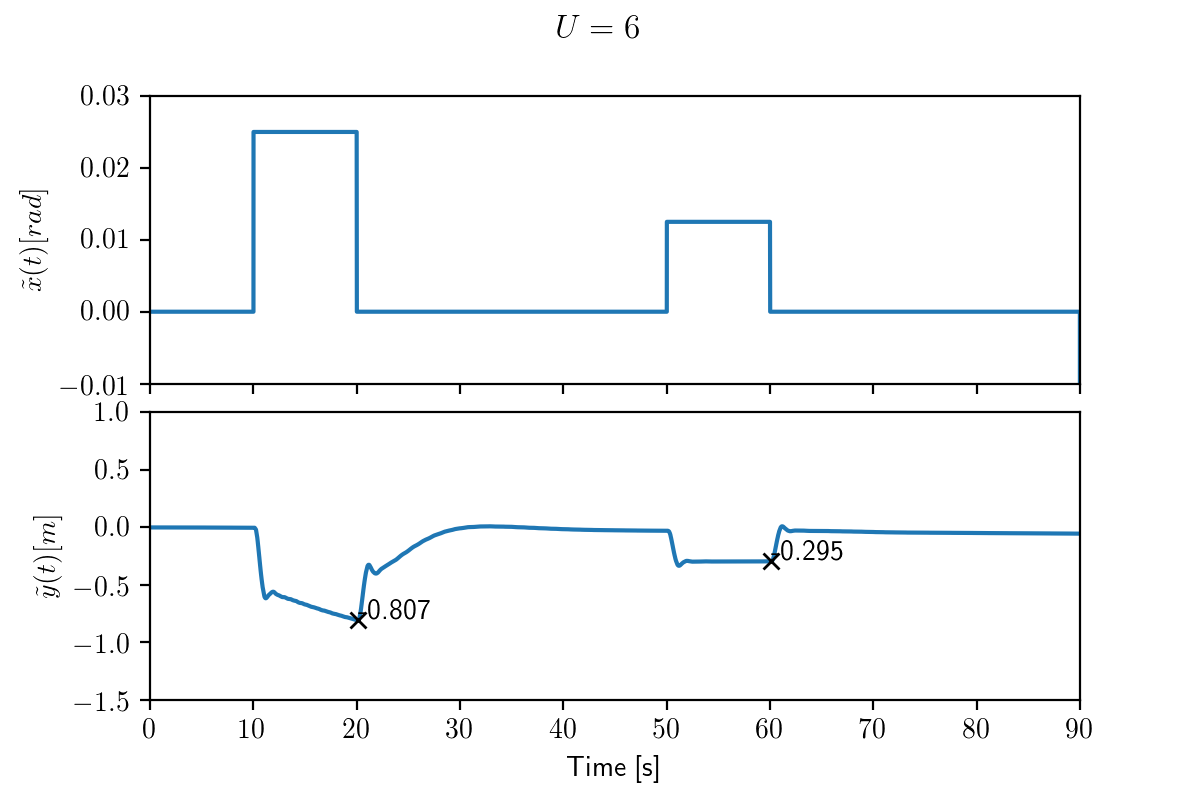
\includegraphics[width=\textwidth]{pitchstep_6.png}
            \caption[Network2]%
            {{\small a}}    
            \label{fig:mean and std of net14}
        \end{subfigure}
        \hfill
        \begin{subfigure}[b]{0.48\textwidth}  
            \centering 
            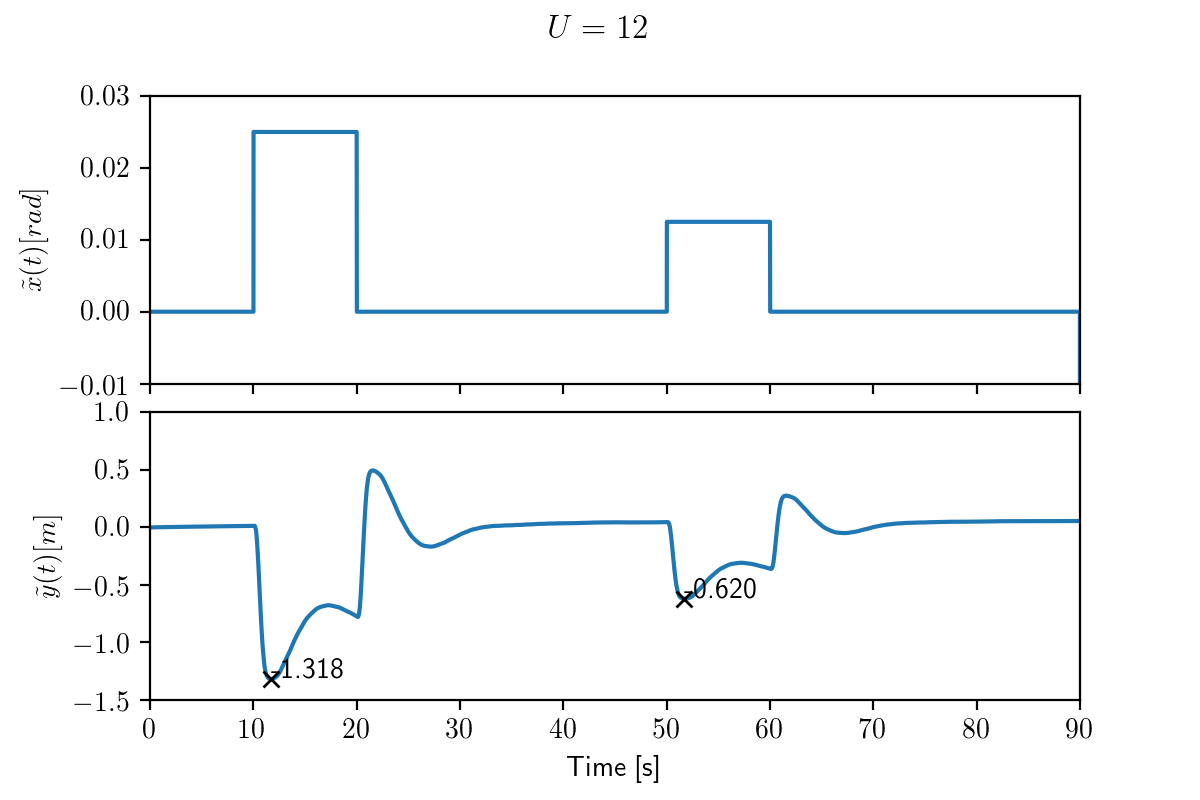
\includegraphics[width=\textwidth]{pitchstep_12.png}
            \caption[]%
            {{\small a}}    
            \label{fig:mean and std of net24}
        \end{subfigure}
        \vskip\baselineskip
        \begin{subfigure}[b]{0.48\textwidth}   
            \centering 
            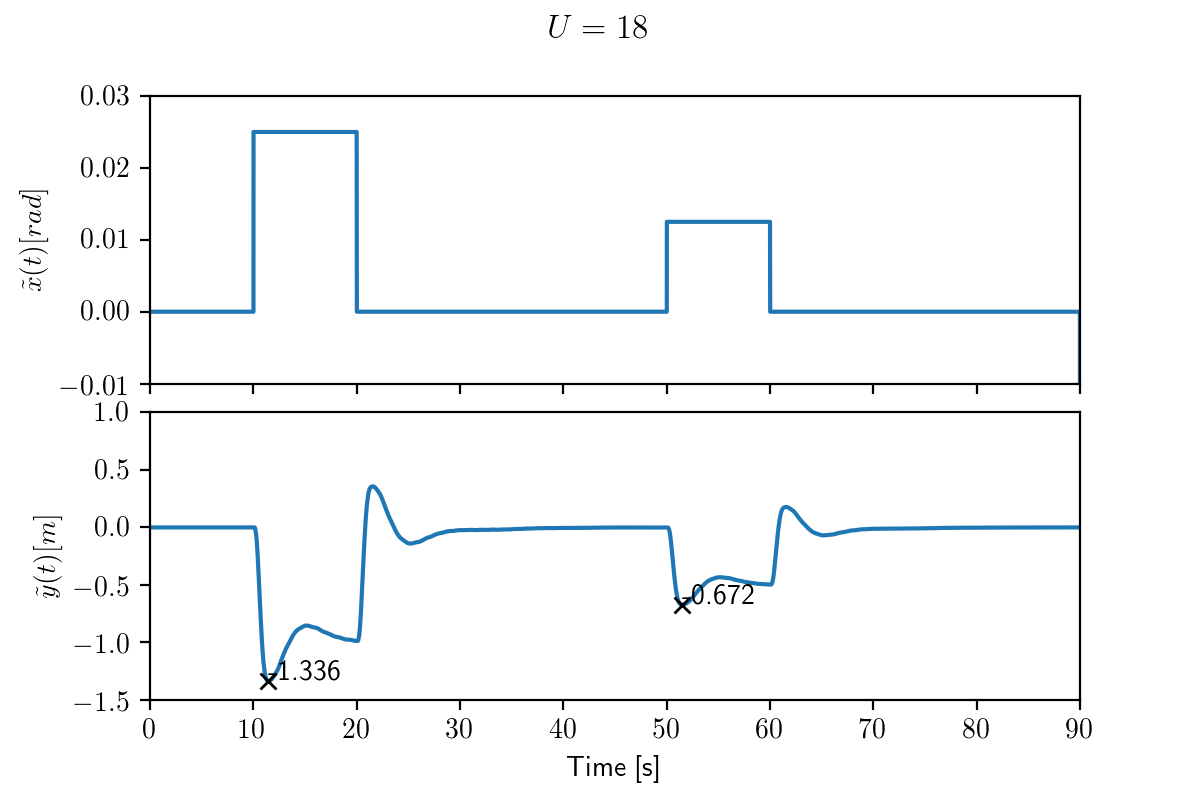
\includegraphics[width=\textwidth]{pitchstep_18.png}
            \caption[]%
            {{\small a}}    
            \label{fig:mean and std of net34}
        \end{subfigure}
        \quad
        \begin{subfigure}[b]{0.48\textwidth}   
            \centering 
            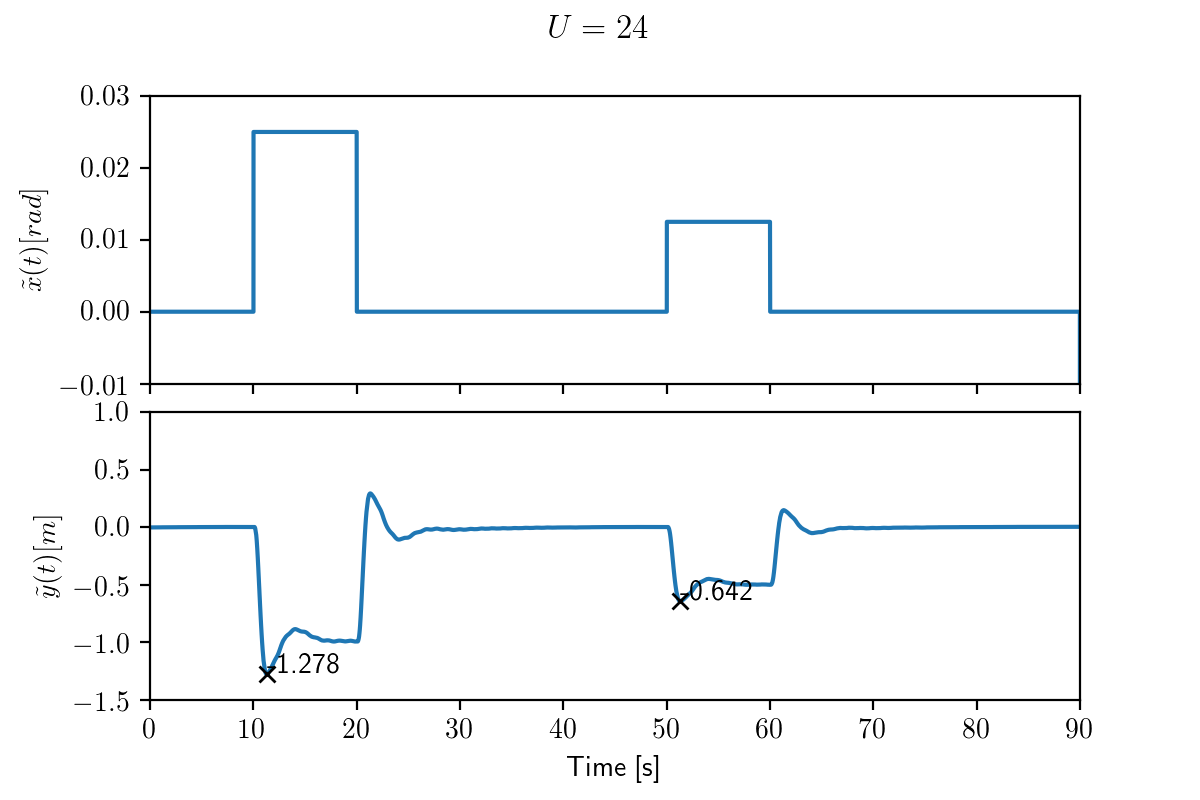
\includegraphics[width=\textwidth]{pitchstep_24.png}
            \caption[]%
            {{\small a}}    
            \label{fig:mean and std of net44}
        \end{subfigure}
        \caption[adsf ]
        {\small asdf} 
        \label{fig:mean and std of nets}
    \end{figure}
    
    
    
    
    
\begin{table}[]
\centering
\caption{My caption}
\label{tab:linearity}
\begin{tabular}{c|ccc}
Windspeed [m/s] & $y_1$  & $y_2$ & $y_1/y_2$ \\ 
\hline
4 & -0.782 & -0.485 & 1.612 \\
6 & -0.807 & -0.295 & 2.736 \\
8 & -0.892 & -0.597 & 1.494 \\
10 & -1.162 & -0.726 & 1.600 \\
12 & -1.318 & -0.620 & 2.127 \\
14 & -1.368 & -0.698 & 1.960 \\
16 & -1.358 & -0.685 & 1.983 \\
18 & -1.336 & -0.672 & 1.987 \\
20 & -1.315 & -0.661 & 1.988 \\
22 & -1.295 & -0.651 & 1.988 \\
24 & -1.278 & -0.642 & 1.990 \\
26 & -1.259 & -0.632 & 1.993 \\
\end{tabular}
\end{table}

\section{Open Loop Output Estimation}
Now that $P$ has been estimated, the spectrum of the open loop output signal is required to be able to design the controller. The open loop output spectrum refers to the frequency decomposition of the flapwise tip deflection for a turbine without tip deflection control. This can be found by running simulations using the DTU10MW turbine with full structural flexibility, realistic aerodynamic effects including wind shear, tower shadow and turbulence. As with the plant model, it is assumed that the output spectrum is a function of operating conditions, and therefore a different spectrum is produced for each wind speed. 3 simulations of 10 minutes each with different turbulent seeds were run for each windspeed. From these simulations, time series data of tip deflection is collected for a particular blade, $i$, for each seed number, $j$, for each wind speed, $U$. For a given wind speed, The tip deflection spectrum, $Y_U(s)$ is by averaging the one sided discrete Fourier transformations, $\mathcal{F}$ for each blade in each seed. That is,

$$Y_U(\omega) = \frac{1}{3N_s}\sum^{3}_{i=1}\sum^{N_s}_{j=1}Y_{U,i,j}(\omega)$$
where the one sided Fourier transform is defined and normalized as:
$$Y_{U,i,j}(\omega)\xleftarrow{\mathcal{F}} \frac{2}{N}\sum^{(N-1)/2}_{n=0}y_{U,i,j}(t) \cdot e^{-n\frac{\omega i}{N}}$$

This particular normalization is chosen so that the frequency component amplitude matches the tip deflection amplitude in meters. In addition to averaging the spectrum over seeds and blades, the spectrum is smoothed by splitting each time series into segments with 256 data points each and taking the average of each of their spectra. Spectra for wind speeds of 6, 12, 18 and 14 $m/s$ are shown in on a log-log plot in Figure \ref{fig:Spectra_OL}. 

\begin{figure}[H]
        \centering
        \begin{subfigure}[b]{0.48\textwidth}
            \centering
            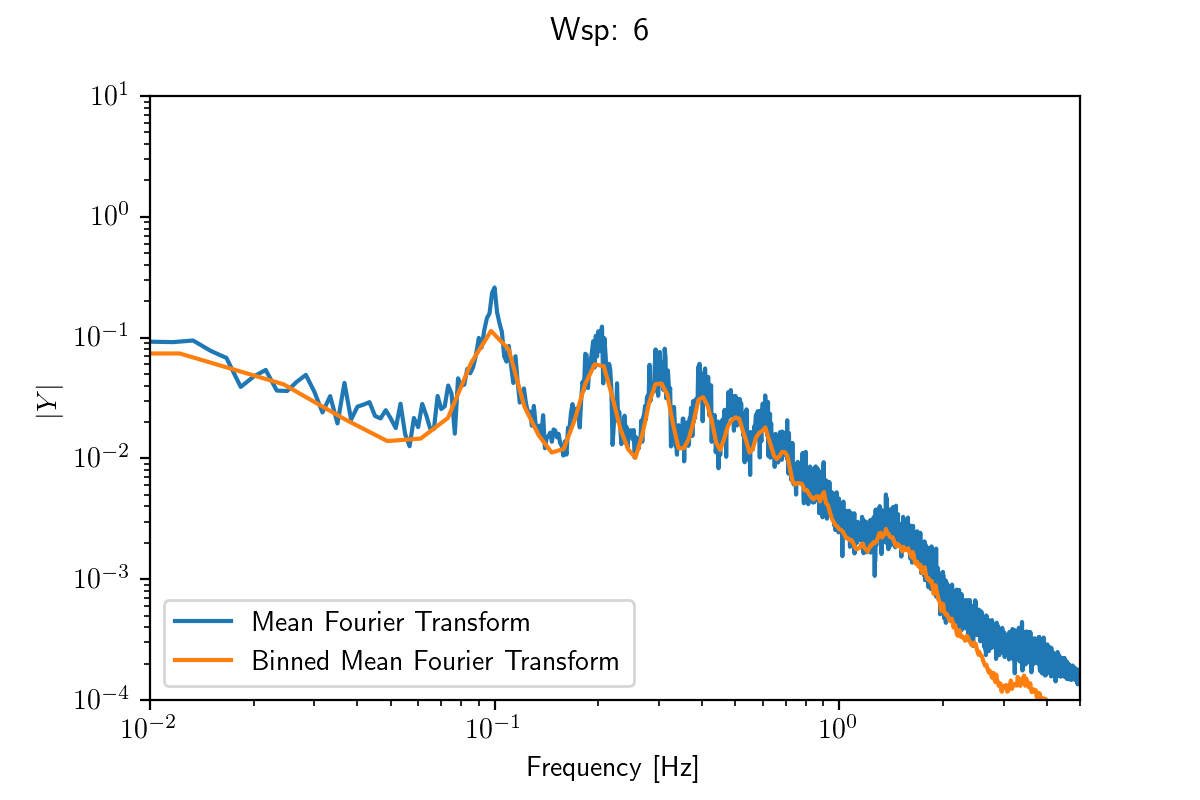
\includegraphics[width=\textwidth]{OLResponse_6.png}
            \caption[Network2]%
            {{\small a}}    
            \label{fig:mean and std of net14}
        \end{subfigure}
        \hfill
        \begin{subfigure}[b]{0.48\textwidth}  
            \centering 
            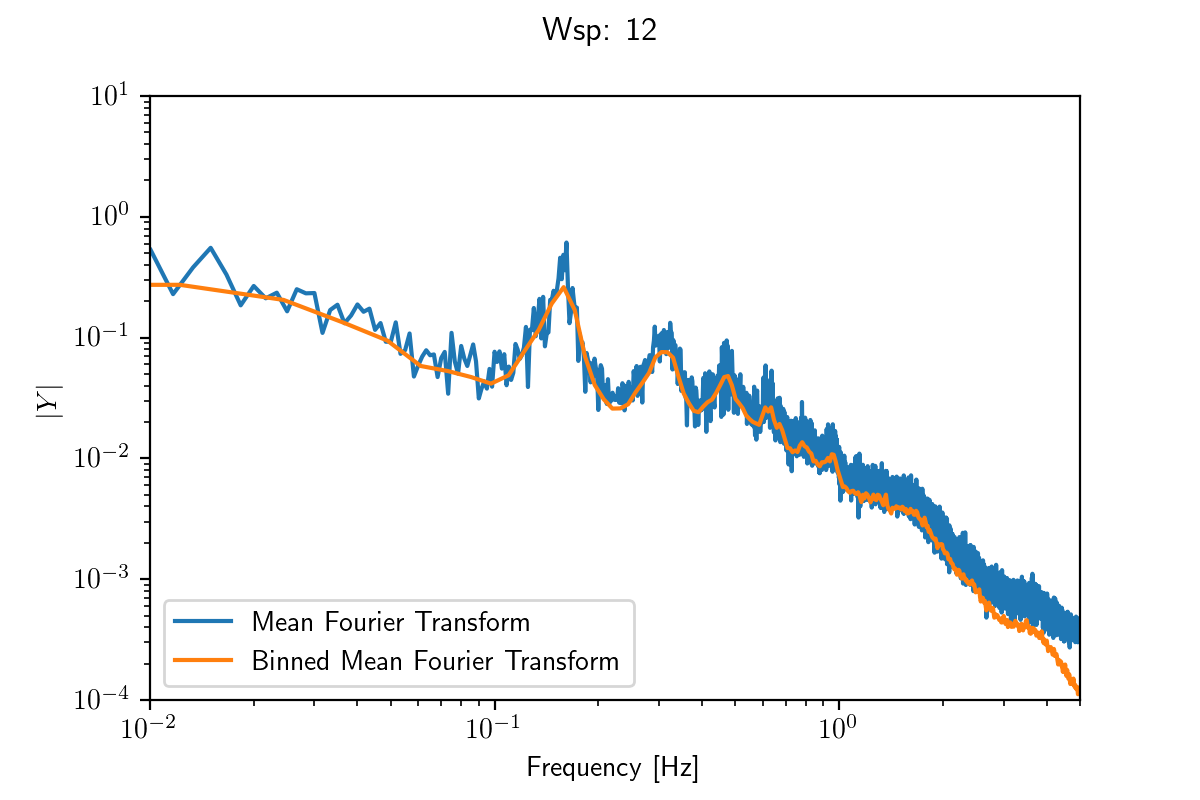
\includegraphics[width=\textwidth]{OLResponse_12.png}
            \caption[]%
            {{\small a}}    
            \label{fig:mean and std of net24}
        \end{subfigure}
        \vskip\baselineskip
        \begin{subfigure}[b]{0.48\textwidth}   
            \centering 
            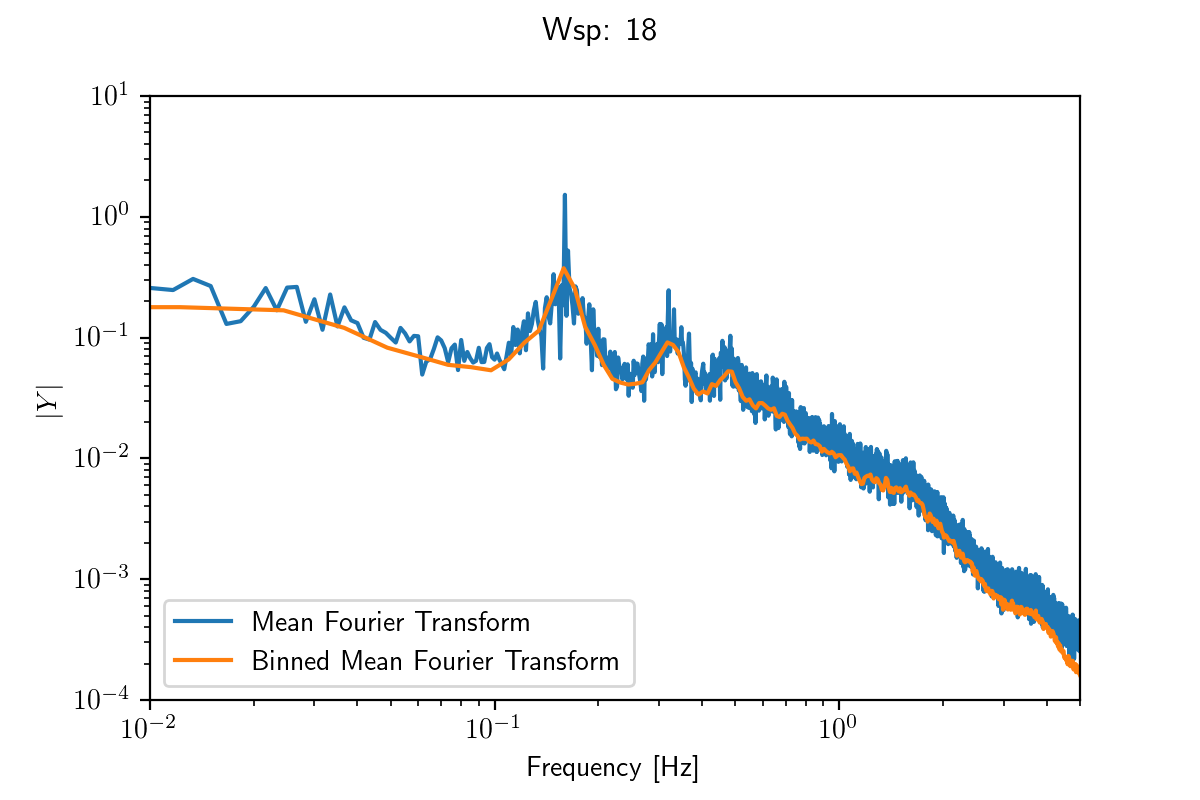
\includegraphics[width=\textwidth]{OLResponse_18.png}
            \caption[]%
            {{\small a}}    
            \label{fig:mean and std of net34}
        \end{subfigure}
        \quad
        \begin{subfigure}[b]{0.48\textwidth}   
            \centering 
            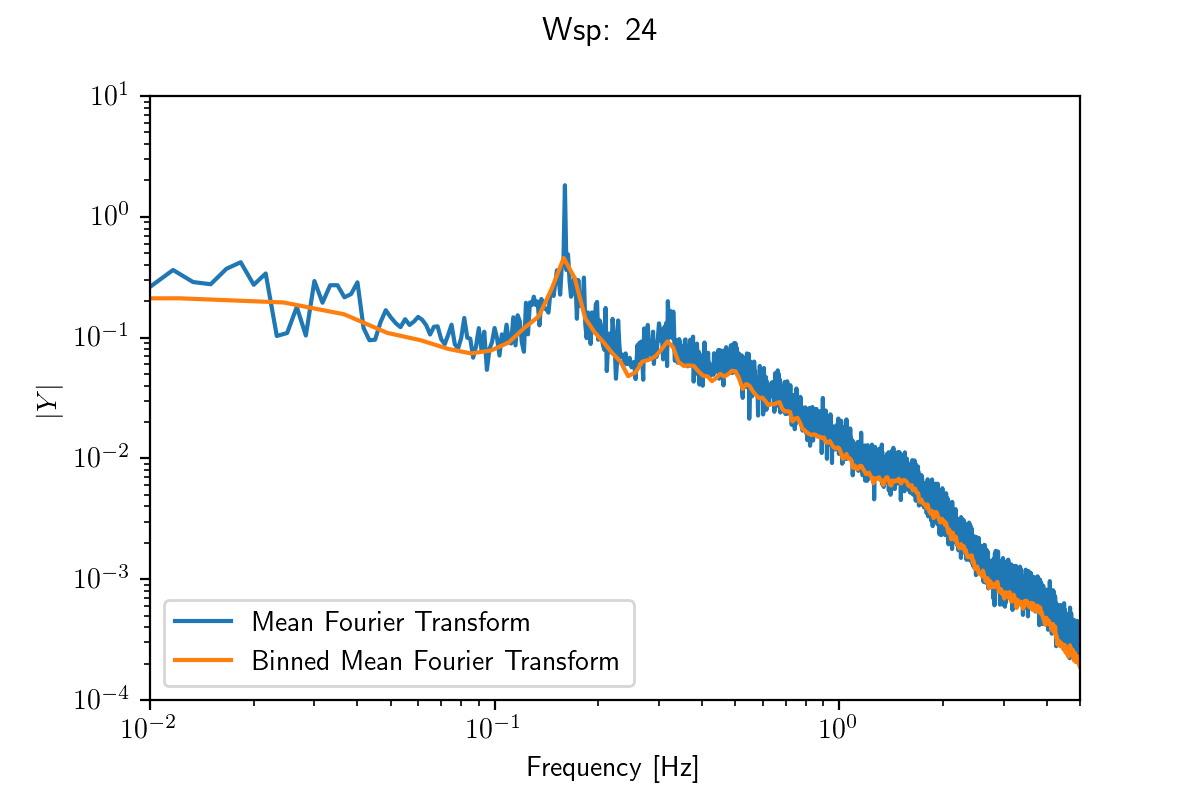
\includegraphics[width=\textwidth]{OLResponse_24.png}
            \caption[]%
            {{\small a}}    
            \label{fig:mean and std of net44}
        \end{subfigure}
        \caption[adsf ]
        {\small asdf} 
        \label{fig:Spectra_OL}
    \end{figure}

\chapter{Tip Disturbance Rejection Controller}
\section{Background}
\subsection{Collective Pitch Control}
Collective pitch control is the basis for turbine power control in modern wind turbines when operating above rated wind speed. Two common objectives are constant torque control or constant power control. Both control objectives are achieved by collectively pitching the turbine blades to control the aerodynamic torque of the rotor. 
\\~\\
It is common to superimpose a high bandwidth controller over the the power/torque controller to decrease the fore-aft tower motion. This is achieved by introducing artificial damping into the tower motion dynamics, reduces fatigue loads in the tower root as well as providing a more stable power output. Control at these frequencies has a much higher bandwidth than the power control loop. Therefore the two controllers are generally superimposed without noticeable interference \cite{15_bossanyi}. \citet{17_Geyler} (check reference), the tower fore-aft damping control is highly coupled with the speed control due to the change in axial wind speed. 

\subsection{Individual Pitch Control}
Although collective pitch and torque control methods can reduce oscillations in the tower and drive train, it is ineffective at reducing certain oscillations in the blades. The reason for this is due to azimuth angle dependent loads such as wind shear and tower shadow. Furthermore, each blade experiences different stresses due to variation in the turbulent structure of the wind field. This is the motivation for individual pitch control (IPC). IPC has shown promising results in literature and simulation, and has only recently been introduced into commercial wind turbines, such as the Vestas V164-9.5.
\\~\\
IPC in literature has shown great reductions in flapwise blade loads using a variety of controller designs. \citet{4_trudnowski} achieved an 86\% reduction in flapwise loads using only the rotor angle as an input signal, however the simulation neglected the effects of turbulence. \citet{5_Bossanyi} showed reductions in equivalent fatigue loads in the out-of-plane (OOP) blade root moments, as well as shaft and yaw bearing moments using IPC compared to CPC. \citet{6_Mirzaei} compared model predictive control and PI control for an IPC system, and found comparable reductions in OOP blade root bending moments in stochastic wind speeds based on LIDAR measurements. \citet{14_Selvam} compares IPC systems using PI control as well as LQG control. PI control achieved load reductions at low frequencies, and the LQG controller was able to achieve load reductions at a higher bandwidth, including 2P and 3P, therefore able to reduce loads on non-rotating parts such as the nacelle, yaw bearing and tower. IPC using~\hinfty control was addressed in \citet{1_Lu}, \citet{2_Kanev} and \citet{17_Geyler}, showing not only reductions in OOP blade root bending moments, but also adequate robustness from unmodelled and stochastic behaviour in the system. In all the considered literature, and to the best of the authors knowledge, load reductions were best achieved in OOP blade root moments rather than in plane moments. The reason for the poor performance of edgewise oscillation control is due to the large magnitude of the gravity loading which can not be avoided easily \cite{4_trudnowski}.
\\~\\
An issue with IPC is the pitch rate of the blades. Pitch rates required to achieve decent reductions in fatigue load are around $\pm10$ deg s$-^1$, which is considered quite high\cite{15_bossanyi}. However, the required pitching rate decreases with rotor diameter due to the decrease in rotational frequency. This justifies the use of IPC for larger wind turbine models. Higher order harmonic control may not meet the limiting pitch rate requirements, which explains why most papers consider low frequency oscillations (usually up to 3P). \cite{17_Geyler}
\\~\\
There are also mechanical concerns regarding the use of IPC. An increase in wear is expected as the pitch must shift at each rotor rotation. Heat dissipation could also be a concern in the pitch actuators, and should be taken into account in the performance of the actuators at different operating temperatures.


\subsection{Active Aerodynamic Load Control}
Active aerodynamic load control (AALC) devices such as trailing edge flaps and micro tabs have also been an active area of research. The advantage of AALC devices is their high bandwidth, allowing for controllability of high frequency dynamics. \citet{7_Berg} and \citet{10_Wilson} have researched the effects of load reduction using trailing edge flaps, showing a 20-32\% reduction in blade root stress, which can allow for a 10\% increase in blade length wihtout exceeding the original equivalent fatigue damage. These papers use tip deflection and tip deflection rate  as controller inputs, making them highly relevant to this the topic at hand. The research in this field is so far restricted to small scale wind turbine models and simulations due to the difficulty and cost of implementing and maintaining such a system on a full scale wind turbine. 





\section{Baseline Control Design}
IPC control is notoriously difficult to compare in literature. There is great variation between the aeroelastic code used, control methodology and wind turbine model. Blade load reduction ranges from 5\% (source) to 85\% (source). 

\subsection{Performance and Robustness}
show performance and robustness for various Kp and Ki and different wind speeds.

\section{Single frequency Control Design}
The first feedback controller to successfully reduce fatigue loads in this project attenuates disturbances at 1P only. This controller consists of a second order low pass filter with a cutoff frequency set at $f_{1P}$, as well as two identical lead compensators:

$$C_{1P}(s) = K\underbrace{\frac{1}{s^2 + 2\zeta\omega s + \omega^2}}_\text{Low pass filter}\underbrace{\frac{(1-aTs)^2}{(1-Ts)^2}}_\text{Lead compensator}$$

The parameters of this controller are defined in Table \ref{tab:C1p_params}. Figure \ref{fig:ipc04_C} shows the bode plot of the controller transfer function. Note that the controller magnitude response peaks at 1P and is highly attenuated at all other frequencies. Furthermore, the phase response at 1P has a phase lead of XXdegrees to account for the lag in the system. 

To do: redo plot to include phase response.
\myFigure[0.7]{ipc04_C.png}{}{fig:ipc04_C}
The full continuous transfer function of this system is:
\begin{equation}\label{eq:C1pa}
C_a = \frac{0.9217s^2 + 0.2030s^1 + 0.0112}{s^4 + 18.4594s^3 + 87.1180s^2 + 27.0252s^1 + 85.1589}
\end{equation}
Using the bilinear transform on Equation \ref{eq:C1pa} for $f_s=100Hz$, the controller is discretised to:


\begin{equation}C_d = \frac{2.1077\times 10^{-5}z^4+4.6387\times 10^{-8}z^3-4.2108\times 10^{-5}z^2  -4.6336\times 10^{-8}z^1  +2.1031\times 10^{-5}}{z^4-3.8234z^3+ 5.4781z^2-3.4861z^1+ 0.8313}
\end{equation}

Todo: represent coefficients in a table instead of a long equation.
Which has the corresponding difference equation:\\
\begin{multiline}
y[k]=2.11\times 10^{-5}x[k]+4.64\times 10^{-8}x[k-1]-4.21\times 10^{-5}x[k-2]-4.63\times 10^{-8}x[k-3]+2.10\times 10^{-5}x[k-4]\\+3.82y[k-1]-5.48y[k-2]+3.49y[k-3]-0.83y[k-4]
\end{multiline}

\begin{table}[H]
\centering
\caption{My caption}
\label{tab:C1p_params}
\label{my-label}
\begin{tabular}{r|l}
\textbf{Parameter}           & \textbf{Value} \\ \hline
Gain, $K$                    & 0.921734          \\
Damping coefficient, $\zeta$ & 0.05           \\
Cutoff frequency, $\omega$   & 1.005          \\
Time constant, $T$           & 0.184          \\
Attenuation constant, $a$    & 29.11         
\end{tabular}
\end{table}

\subsection{Load contributions for $f_{np}$ for $n=1,2,3,4$}




\section{$f_{1p}$ and $f_{2p}$ Control Design}

\section{Performance in Normal Turbulence}

\section{Performance in Extreme Turbulence}

\section{Performance in Inverse Shear}


\myFigure[0.7]{ipc04_OL_CL_bode.png}{}{fig:ipc04_OL_CL}
\myFigure[0.7]{ipc04_S.png}{}{fig:ipc04_S}
\myFigure[0.7]{ipc04_L.png}{}{fig:ipc04_L}
\myFigure[0.7]{ipc04_nyquist.png}{}{fig:ipc04_nyquist}







\chapter{Tip Trajectory Tracking Controller}
\input{Chapters/Tip_Trajectory_Tracking.tex}

\chapter{Things I have Written But Haven't Integrated in The Report Properly}
\section{Literature Review}

\subsection{Background}
Since the advent of modern wind turbine design, the capacity and size of wind turbines has increased dramatically. From the first electricity-producing wind turbine with a rotor diameter of 17m, the design trend has shown huge growth in rotor size with a 180m rotor on the Adwen 8MW platform. As the size of wind turbines continues to increase, new challenges arise in terms of rotor aerodynamics, structural design and control. large rotors require slender, lighter blades to maintain aerodynamic efficiency and to combat the increase in manufacturing costs. This comes at the cost of exacerbated fatigue loads as the blades experiences various forces as they sweep around the rotor plane.
\\~\\
It is well known in the wind industry that loads induced by gravity loads, tower shadow, wind shear, turbulence and gusts can cause significant damage to the blade roots, rotor shaft and the tower \cite{13_Dolan}. By introducing a larger rotor, not only is the turbine more susceptible to this damage, but new instabilities can also be introduced such as aeroelastic flutter, whirling modes, and dynamic coupling such as tower tilt-yaw and blade flap-torsion coupling \cite{7_Berg}.
\\~\\
These problems are typically addressed in the aerodynamic and structural design of the wind turbine to ensure significant damage does not occur by introducing safety factors and increasing blade strength. It is becoming increasingly difficult to both predict the effect of these weaknesses and instabilities as well as effectively eliminate them in the design stage without incurring costs in other aspects of the design, such as increased blade mass. For this reason, the wind industry is focusing more attention on innovative methods for reducing loads. One method, which is the focus of this thesis, is the use of active control methods to actively mitigate fatigue loads in order to extend the lifespan of wind turbine components. In particular, the use of tip deflection sensors in a control system will be investigated.
\\~\\
\subsection{Fatigue Load Mitigation in Wind Turbine Control Systems}
The concept of active load control is not a new concept in the wind industry. Tower and drive train loads can successfully be reduced by extending the basic speed control used in modern variable speed wind turbines.
\subsubsection{Torque Control}
Torque control is used to maintain optimal power output when the wind turbine is operating below rated wind speed. The idea is to balance the aerodynamic and generator torque to achieve a maximum power coefficient $C_p$. A common control strategy to achieve this is to use a proportionality relationship between demanded torque $Q$, and the square of the generator angular velocity $\omega_g$
$$Q = \frac{\pi \rho R^5 C_p}{2\lambda^3 G^3}\omega_g^2$$ \cite{15_bossanyi}

torque control has also been used to introduce side-side tower damping and mitigate drive train torsion vibration. WRITE MORE
\subsubsection{Collective Pitch Control}
Collective pitch control is the basis for turbine power control in modern wind turbines when operating above rated wind speed. Two common objectives are constant torque control or constant power control. Both control objectives are achieved by collectively pitching the turbine blades to control the aerodynamic torque of the rotor. 
\\~\\
It is common to superimpose a high bandwidth controller over the the power/torque controller to decrease the fore-aft tower motion. This is achieved by introducing artificial damping into the tower motion dynamics, reduces fatigue loads in the tower root as well as providing a more stable power output. Control at these frequencies has a much higher bandwidth than the power control loop. Therefore the two controllers are generally superimposed without noticeable interference \cite{15_bossanyi}. \citet{17_Geyler} (check reference), the tower fore-aft damping control is highly coupled with the speed control due to the change in axial wind speed. 

\subsubsection{Individual Pitch Control}
Although collective pitch and torque control methods can reduce oscillations in the tower and drive train, it is ineffective at reducing certain oscillations in the blades. The reason for this is due to azimuth angle dependent loads such as wind shear and tower shadow. Furthermore, each blade experiences different stresses due to variation in the turbulent structure of the wind field. This is the motivation for individual pitch control (IPC). IPC has shown promising results in literature and simulation, and has only recently been introduced into commercial wind turbines, such as the Vestas V164-9.5.
\\~\\
IPC in literature has shown great reductions in flapwise blade loads using a variety of controller designs. \citet{4_trudnowski} achieved an 86\% reduction in flapwise loads using only the rotor angle as an input signal, however the simulation neglected the effects of turbulence. \citet{5_Bossanyi} showed reductions in equivalent fatigue loads in the out-of-plane (OOP) blade root moments, as well as shaft and yaw bearing moments using IPC compared to CPC. \citet{6_Mirzaei} compared model predictive control and PI control for an IPC system, and found comparable reductions in OOP blade root bending moments in stochastic wind speeds based on LIDAR measurements. \citet{14_Selvam} compares IPC systems using PI control as well as LQG control. PI control achieved load reductions at low frequencies, and the LQG controller was able to achieve load reductions at a higher bandwidth, including 2P and 3P, therefore able to reduce loads on non-rotating parts such as the nacelle, yaw bearing and tower. IPC using~\hinfty control was addressed in \citet{1_Lu}, \citet{2_Kanev} and \citet{17_Geyler}, showing not only reductions in OOP blade root bending moments, but also adequate robustness from unmodelled and stochastic behaviour in the system. In all the considered literature, and to the best of the authors knowledge, load reductions were best achieved in OOP blade root moments rather than in plane moments. The reason for the poor performance of edgewise oscillation control is due to the large magnitude of the gravity loading which can not avoided easily \cite{4_trudnowski}.
\\~\\
An issue with IPC is the pitch rate of the blades. Pitch rates required to achieve decent reductions in fatigue load are around $\pm10$ deg s$-^1$, which is considered quite high\cite{15_bossanyi}. However, the required pitching rate decreases with rotor diameter due to the decrease in rotational frequency. This justifies the use of IPC for larger wind turbine models. Higher order harmonic control may not meet the limiting pitch rate requirements, which explains why most papers consider low frequency oscillations (usually up to 3P). \cite{17_Geyler}
\\~\\
There are also mechanical concerns regarding the use of IPC. An increase in wear is expected as the pitch must shift at each rotor rotation. Heat dissipation could also be a concern in the pitch actuators, and should be taken into account in the performance of the actuators at different operating temperatures.


\subsubsection{Active Aerodynamic Load Control}
Active aerodynamic load control (AALC) devices such as trailing edge flaps and micro tabs have also been an active area of research. The advantage of AALC devices is their high bandwidth, allowing for controllability of high frequency dynamics. \citet{7_Berg} and \citet{10_Wilson} have researched the effects of load reduction using trailing edge flaps, showing a 20-32\% reduction in blade root stress, which can allow for a 10\% increase in blade length wihtout exceeding the original equivalent fatigue damage. These papers use tip deflection and tip deflection rate  as controller inputs, making them highly relevant to this the topic at hand. The research in this field is so far restricted to small scale wind turbine models and simulations due to the difficulty and cost of implementing and maintaining such a system on a full scale wind turbine. 
\subsection{Sensing methods}
Real time measurements have become increasingly important for wind turbines and wind farms over recent years, allowing for sophisticated digital control. The stream of data is typically referred to as Supervisory control and data acquisition (SCADA), and can comprise of a variety of novel measurements from components of the turbine. A summary of sensors relevant to active load reduction is described in this section.
\subsubsection{Rotor Azimuth measurement}
Modern wind turbines use rotor angular velocity for the power control loop rather than the rotor azimuth angle. For IPC, a measurement of the rotor azimuth angle is vital in transforming the rotor frame of reference to the fixed tower frame of reference. This is because many load oscillations are dependent on the azimuth angle, such as tower shadow, wind shear and yaw misalignment. 
\\~\\
\citet{4_trudnowski} demonstrated effective control of flap wise loads given only the rotor azimuth angle. Given a precise model of how the wind field varies with rotor angle, for example, \citet{13_Dolan}, this type of control can be possible. However,the wind field can vary dramatically for a given site, and therefore a controller using only rotor azimuth angle would likely be ineffective in the real world. Additionally, fluctuations due to turbulence can not be effectively reduced without additional sensing and controller feedback. Nevertheless, the use of rotor azimuth sensing in conjunction with additional sensors is relevant to this project.

\subsubsection{Wind measurements}
Cup anemometers and wind vane are the standard, IEC-approved method for taking wind speed and direction measurements, however they are unable to capture high frequency components of the wind field as well as spacial variation. As with the power control, load reduction controllers can benefit from the low frequency cup anemometer measurements for gain scheduling. Wind fields can vary greatly over time and space, more advanced sensors may be beneficial to observe how the wind field varies with rotor azimuth angle. LIDAR measurements can provide wind field data at both a high frequency and spacial resolution, and can provide useful information to a control system regarding gusts and field variations before they are experienced by the turbine. \citet{6_Mirzaei} Demonstrated that model predictive control methods were more effective than PI control when used with upstream LIDAR measurements especially in transitioning wind conditions. 
\\~\\
Although the wind measurement techniques is beyond the scope of this project, it should be noted that tip deflection sensors could provide useful information in terms of gust control when used in conjunction with wind speed measurements. \citet{2_Kanev} uses blade root bending moment measurements, both in-plane and out-of-plane, in order to better estimate the blade-effective wind speed, and to additionally detect gust events. An extended Kalman filter observer was used as a nonlinear observer for this study.
\\~\\
...
\subsubsection{Tower Acceleration}
Tower motion, both in the fore-aft and side-side direction, is the source of fatigue loading in the tower. Additionally, the fore-aft dynamics of the tower is coupled with the power output of the turbine due fluctuations in the effective wind speed at the rotor. For this reason, tower damping is often a control objective using pitch and torque control. In order to effectively reduce this oscillation, measurements of the tower acceleration are generally used as feedback to the control system. This can easily be performed with an accelerometer in the nacelle of the wind turbine \cite{15_bossanyi}.
\subsubsection{Strain Gauges}
Commonly used in literature for IPC. No apparent reason for using strain gauges over tip deflection sensors. will write more here.
\subsubsection{Tip Deflection Sensors}
Tip deflection sensors are not commonly cited in literature. Bossanyi briefly mentions the possibility of using accelerometers in the blade tips as an alternative to strain gauges, and also mentions the difficulty of maintaining such sensors due to inaccessibility of the blade tips. \cite{5_Bossanyi} \cite{15_bossanyi}. \citet{7_Berg} and \citet{10_Wilson} use tip deflection sensors in their turbine controller designs, however they focus on active flap control. To the best of the author's knowledge, no research has been performed on IPC using tip deflection sensors instead of strain gauges. using \textcolor{red}{A whitepaper on the cost benefits and basic implementation of the iRotor would be very nice in this section}.
\subsection{Wind Turbine Modelling}
\textcolor{red}{will elaborate on this section}
\subsubsection{Structural}
Something on Euler-Bernoulli beam theory vs Timoshenko, and that HAWC2 uses Timoshenko. Something about the simplified structural models(usually 1 mode for blades and tower) used in literature, and the different assumptions they make and why. Usually a simplified model will suffice and provides transparency to the controller.
\subsubsection{Aerodynamic Modelling}
Aerodynamic models can be complicated (CFD, actuator models), difficult to implement in a control system. Can use advanced models to get linear approximations of system dynamics. Talk about how this is addressed in literature for IPC.
\cite{11_Wang}

\subsection{Observer design}
Kalman filter \cite{15_bossanyi}, extended kalman filter \cite{2_Kanev}. Implementation, and inclusion of colored wind spectrum \cite{14_Selvam}. 
\\
A fundamental aspect of a wind turbine controller is the state observer. The state observer recreates the structural and aerodynamic state of the wind turbine system. A good observer is able to improve controller response by providing a short term prediction how the state will change. It is able to track the state precisely over different working conditions, and in the presence of noise, both from the measurements and from the system dynamics itself. A standard and highly effective observer design is typically the Kalman filter. A Kalman filter is able to DESCRIBE THE KALMAN FILTER. In linear control theory, a Kalman filter is straight forward to design if the process and measurement noise can be known a priori. The Kalman filter can be extended to nonlinear systems by using an extended Kalman filter, which uses a linearized approximation of the current operating point. Something about the unscented Kalman filter. Something about a second order extended Kalman filter (augmented Kalman filter) (maybe not?).
\\~\\
An alternative and novel approach to state observation is using machine learning algorithms. WRITE ABOUT THIS
\subsection{IPC Controller design}
As the control problem at hand is nonlinear, there are a number of controller designs which have been proposed in literature regarding IPC. One common step is performing a transformation to convert the system into a time invariant system. This is called the Coleman transformation, which is a special case of the the multi-blade coordinate transformation, and also known as the d-q transformation borrowed from electrical machine theory. The Coleman transformation removes the dependency of rotor azimuth angle from the system, allowing for linear control methods to be used. More specifically, the Coleman transformation converts the flapwise and edgewise loads into tower tilt and yaw moment, effectively representing 3P loads (or is it 1P?) into 0P loads. In addition to the Coleman transformation, many control ideologies have been adopted in literature. Some of the more common methods are outlined in the following section.

\subsubsection{PI Control}
PI control is the most basic control method used in literature. PI control is a linear control method which provides a control signal proportional to to the error signal and its integral over time. When used in IPC, it is assumed that the yaw and tilt moment decomposition resulting from the Coleman transformation are decoupled. This allows the tilt and yaw to be treated independently with two separate PI controllers. PI control is often used as a benchmark for testing other control methods in IPC. Despite the simplicity of the control method, it shows comparable results to more advanced models at low bandwidths and is more transparent in its implementation \cite{6_Mirzaei}, \cite{14_Selvam}. 
\\~\\
The underlying assumption of using PI control for IPC is the decoupling between the tilt and yaw degrees of freedom. In reality, this is not the case. \citet{1_Lu} presents the weaknesses of the decoupling assumption. Additionally, performing the Coleman transformation and its inverse causes a frequency shift in the system dynamics which should be taken into account in the controller design. 
\subsubsection{Linear-Quadratic-Gaussian Regulator}
A linear-quadratic-Gaussian regulator (LQG) is a multi-input-multi-output (MIMO) control method that provides optimal control to uncertain linear system with white noise disturbances. A LQG is a combination of a linear-quadratic regulator (LQR) with a Kalman filter as a state estimator. For a linear system, the LQR and the Kalman filter can be designed independently of each other. The controller is able to act on multiple sensor inputs and achieve multiple control objectives by changing the weights of a cost function.  \citet{14_Selvam} and \citet{5_Bossanyi} use LQG, and it works pretty well (elaborate more).
\\~\\
The weakness of LQG is that it is a linear controller, which means that it may not perform well on the nonlinear dynamics of a wind turbine. This can usually be addressed by linearising the system about control points and with gain scheduling.
\subsubsection{\hinfty Loop Shaping}
\hinfty loop shaping is a control technique conducted in the frequency domain, where the frequency response of a system can be adjusted through optimisation. \hinfty loop shaping had the advantage of being able to include robustness in its control objective. My understanding of \hinfty loop shaping is a bit rusty. Will elaborate later. 

Used in \cite{1_Lu} to overcome the tilt-yaw coupling problem in PI control. Used in \citet{17_Geyler} on a simple wind turbine model. The unmodelled behaviour is taken into account in the robustness of the \hinfty controller. Also successfully used in \citet{2_Kanev}.
\subsubsection{Model Predictive Control}
Model predictive control used in \cite{6_Mirzaei}.
\subsubsection{Machine Learning}

Neural networks and machine learning. \cite{8_Wang} \cite{3_Treiber}. bad because black box, and does not add any benefits over modern control theory. the motivation is lacking according to \citet{15_bossanyi}

...Cyclic pitch control - Selvam.



% The unique aspect of this paper is in the use of tip deflection sensors instead of a strain gauge at the blade roots. This has rarely been investigated in literature. \citet{7_Berg} addresses the use of tip deflection readings as an input for a turbine control system using active flaps. DESCRIBE RESULTS. Although active flaps can provide a high frequency response for a turbine controller, they have yet to be used in commercial turbine models, and are typically reserved for academic research. Active flaps are expected to increase operating and maintenance costs due to the additional moving parts required. XX mentions the possibility of using tip deflection readings as an alternative input. Apart from these references, tip deflection sensors have not been largely considered in literature to the best of the author's knowledge. It follows that the use of tip deflection sensors in conjunction with IPC has not been explored, and will remain the focus of this paper.
% \\~\\
\textcolor{red}{Not sure where to write a section on the types of loads, or what to cite.
Two types of loads are typically considered in engineering design: fatigue load and ultimate load. Fatigue loads occur as a result of structural oscillations over a long period of time. Calculations relating to fatigue largely consider the magnitude of the loading rather than the frequency. The rainflow counting algorithm developed by XX, is commonplace in engineering in distinguishing the the number of cycles of different magnitudes in a timeseries. Using the rainflow counting results, a short term equivalent load can be determined using BLAH BLAH. An equivalent load is a way of representing the fatigue load, which may consist of various amplitude oscillations at different frequencies, as a single sinusoidal oscillation with a fixed frequency (typically 1Hz). One control objective could be to minimise the short term equivalent load of the wind turbine blades over the operating lifetime.
\\~\\ 
The second type of load that is considered is the ultimate load, which is the largest expected load to occur over a short period of time. Extreme loads which exceed the ultimate strength of a component can lead to instantaneous catastrophic failure of a wind turbine, and can occur due to extreme winds or gusts. IEC standards consider the most extreme load within a 10 minute period which is expected to occur over 50 year time period. Extreme analysis, such as the use of a Gumbel distribution is commonly used to predict the 50 year extreme load based on limited time series data.}
\\~\\
\textcolor{red}{Take into account torsion?
\citet{7_Berg} says flap bending - torsion coupling increases with rotor sizze. ignores torsion as impact is minor. }
\\\textcolor{red}{Is cyclic pitch control the same as IPC? Should I make a distinction?}
\\
\textcolor{red}{Is a sensor to measure azimuth angle the same as the sensor used to measure rotor speed? }\\
\textcolor{red}{What are the benefits of using tip deflection sensors}

\section{Theoretical Content and Methodology}
\subsection{Relationship between Tip Deflection and Blade Loads}
In order to reduce blade loads with tip deflection control, a relationship between blade loads and tip deflection must exist. In particular, bending moment at the blade root is of interest as this is where the largest load occurs. In order to show a relationship analytically, a simplified structural model of a wind turbine blade is presented in this section. It should be noted that loads and deflection in the flapwise direction is considered. 
\\~\\
The blade is assumed to behave as an Euler-Bernoulli cantilever beam with length $L$ and uniform bending stiffness, $EI$. The flapwise deflection of the beam, $u(t, z)$, at a distance, $z$, and at a time, $t$, from the fixed end, can be expressed a linear combination of the mode shapes:

\begin{equation}
    u(t, z) = \sum_{i=1}^\infty \alpha_i(t) \gamma_i(z)
\end{equation}
where $\alpha_i$ is the amplitude of the $i$th mode, and $\gamma_i$ is the non-dimensional shape of the $i$th mode. $\gamma_i(z)$ is normalized such that its value at the tip is 1. That is, $\gamma_i(L) = 1$. Therefore, $\alpha_i$ has units of distance and can be interpreted as the tip deflection distance contribution for the $i$th mode. That is,
\begin{equation}
    u(t, L) = \sum_{i=1}^\infty \alpha_i(t)
\end{equation}
\\
From Euler-Bernoulli beam theory, the bending moment, $M(z)$, is expressed as:
\begin{equation}
    M(z) = EI(z)\frac{\partial ^2 u}{\partial z^2}(z)
\end{equation}
Where $EI$ is the flexural rigidity defined as the product of the area moment of inertia and the Young's Modulus of the beam material. Substituting XX into XX, and noting that $\alpha_i$ is invariant to transverse displacement, the expression for $M(z)$ becomes:
\begin{equation}
    M(z) = EI(z)\sum_{i=1}^\infty \alpha_i(t)\frac{\partial ^2 \gamma_i}{\partial z^2}(z)
\end{equation}
     
Now assume only the first flapwise mode is relevant and consider the contribution from all higher modes as negligible. That is, assume:
\begin{equation}
    u(t, z) \approx  \alpha_1(t) \gamma_1(z)
\end{equation}
From XX, and XX, the tip deflection $y(t)$ and the root bending moment, $M(t)$, can be related by:
\begin{equation}
    M(t) = EI(0)\left.\frac{\partial ^2 \gamma_i}{\partial z^2}\right\vert_{z=0}y(t)
\end{equation}
Or put another way, the proportionality between tip deflection and root bending moment is:
\begin{equation}
    \frac{y(t)}{M(t)} = \frac{1}{EI(0)\left.\frac{\partial ^2 \gamma_i}{\partial z^2}\right\vert_{z=0}}
\end{equation}
From the specifications of the DTU10MW turbine, this proportionality constant can be approximated. The first modal shape is determined using the eigenvalue solver in HAWC2, which provides $\gamma_i(z)$. A spline is fit to $\gamma_1(z)$, which is then numerically integrated twice and evaluated at $z=0$ to get the curvature at the root. Using the parameters in Table xx to evaluate Equation XX, the proportionality between tip deflection and RBM is estimated to be $y(t)/M(t) = 3.827 \times 10^{-7} m/Nm$. In section XX, this result is validated and shows that the actual proportionality is higher due to the unmodelled dynamic effects.

\begin{table}[H]
\centering
\caption{My caption}
\label{my-label}
\begin{tabular}{r|l}
\textbf{Parameter} & \textbf{Value} \\ \hline
$E(0)$         & $ 1.2612\times 10^{10}$ $Nm^{-2}$   \\
$I(0)$         &     $4.8374 m^4$  \\
   $\left.\frac{\partial ^2 \gamma_i}{\partial z^2}\right\vert_{z=0} $     &    $4.2827\times 10^{-5} m^{-2}$  
\end{tabular}
\end{table}
\\~\\
% THIS IS WRONG
% In the case that the beam is statically loaded with a point force, $p$ at the tip, then the root moment, $M(0)$ and tip deflection, $x(L)$ can be expressed as:
% $$M(0) = pL$$
% $$x(L) = \frac{pL^3}{3EI}$$
% which leads to the expression:
% $$x(L) = \frac{L^2}{3EI}M(0)$$
% Similarly, in the case that the beam is uniformly loaded with force per unit length, $q$, then $M(0)$ and $x(L)$ can be expressed as:
% $$M(0) = \frac{qL^2}{2}$$
% $$x(L) = \frac{qL^4}{8EI}$$
% which leads to the expression:
% $$x(L) = \frac{L^2}{4EI}M(0)$$

% Note how in both cases, $x(L)$ is proportional to $M(0)$ and the proportionality is independent of the magnitude of the load. As the force distribution of a typical turbine blade increase along the length of the blade, the actual relationship between tip deflection and root bending moment is likely similar to the two cases presented above. In other words, the proportionality constant between tip deflection and root bending moment for a static blade is likely in the range:
% $$\frac{L^2}{4EI} < \frac{x(L)}{M(0)} < \frac{L^2}{3EI}$$

% From the specifications of the DTU10MW turbine, the range of flapwise proportionality constants can be estimated. The length of the blades from blade root to tip is $86.366m$. The stiffness of the blade varies along its length. So an equivalent flapwise stiffness $\overline{EI}=1.1\times 10^{10} Nm^{-2}$ is determined in Appendix XX (To do). From these values, it is estimated that the proportionality is in the range:
% $$1.7 \times 10^{-7} < \frac{x(L)}{M(0)} <  2.2\times 10^{-7} \qquad m/Nm$$
% It should be noted that this model assumes the load is static, which is not the case for the fluctuating blade loads. In section XX, this result is validated and shows that the actual proportionality is higher due to the unmodelled dynamic effects.
%ASSUMPTIONS (tower shadow, wind shear, etc)
%\\~\\
%The system identification package in MATLAB is used to estimate the transfer function. A fit percentage is given to each fit using the Normalized Root Mean Squared Error (NRMSE), defined as
%$$\text{NRMSE}=\left(\frac{\norm{x_{\text{meas}}-x_{\text{model}}}_2}{\norm{x_{\text{meas}}-\overline{x_{meas}}}_2}\right)$$
%Results show that a transfer function with 2 poles and 1 zero is adequate for representing the relationship between tip deflection and bending moment compared to other linear systems. This implies a relationship between the tip deflection rate and a second order system describing root bending moment:
%$$a\ddot{M} + b\dot{M} + cM = \dot{x}_{td}$$

\subsection{Quantifying Fatigue Loads}
The turbine simulations produce complicated time histories of the loads experienced in the various components of the turbine. In order to quantify and compare the fatigue damage experienced in these components, a load spectrum is calculated. A load spectrum decomposes a complicated stress history into stress cycles of varying amplitude. This can be achieved using rain flow counting \cite{matsuishi1968fatigue}. The fatigue loads in the turbine components can be quantified by calculating the equivalent load at 1Hz. The equivalent load is the amplitude of a 1Hz oscillating load which produces the same amount of fatigue damage to a component as a mixed load spectrum. It is a way of comparing different load spectra of the same component. The Equivalent load (Note: abbreviate to DEL instead of S_eq), $S_{eq}$, is calculated for $N_{eq}$ cycles as follows:

\begin{equation}\label{eq:DEL}
S_{eq} = \left(\frac{\sum_i N_iS_i^m}{N_{eq}}\right)^{\frac{1}{m}}
\end{equation}

Where $S_i$ is the $i$th load cycle amplitude, $N_i$ is number of full cycles at $S_i$, $m$ is the material W\"{o}hler curve exponent of the component in question. In this analysis, a W\"{o}hler curve exponent of 4 and 10 is used for steel (tower, rotor shaft, etc) and composite materials (ie. rotor blades) respectively. $N_eq$ is the number of cycles experienced of load $S_{eq}$. For 600 second simulations, which is the case for this analysis, A 1Hz equivalent load requires $N_{eq}=600$. It can be observed from Equation \ref{eq:DEL} that the damage equivalent load is highly sensitive to large amplitude oscillations due to the exponentiation of the W\"{o}hler curve exponent. Therefore even a small reduction in load amplitudes can lead to large reduction in lifetime fatigue loads in the turbine components.



\subsection{Disturbance Rejection Theory}

Unlike the the collective pitch controller, which aims to minimise the error between the power output and a target power output, the task of an IPC is disturbance rejection. Consider the linear feedback system in Figure XX. Frequency components of the disturbance signal, $D(s)$ are passed through to the output, $Y(s)$ described by the closed loop transfer function, $G(s) = P(s)/(1+P(s)C(s))$ 

\ref{fig:analModel:4}. The closed loop transfer function reveals fundamental design parameters in this disturbance rejection.
\begin{itemize}
\item Disturbances are attenuated when the denominator of $G(s)$ is large.
\item Disturbances are passed through to the output signal when the denominator is small.
\item the $G(s)$ is unstable when the denominator equals zero.
\end{itemize}
To perform well, the denominator of the system should be large at the frequency it wishes to reject. In other words, $P(s)C(s)$ should be large for an $s$ corresponding to the desired frequency to reject. For robustness and stability, the denominator of the blade system should not be equal to zero. Measures of performance and robustness in a disturbance rejection control system are outlined in the following sections.

\subsection{Performance Measures for Disturbance Rejection}
The objective of the controller is to attenuate the effect of disturbances, $d(s)$ on the system output, $x(s)$. One way of measuring the effectiveness of a disturbance rejection control system is to compare the outputs of two systems: the open loop system (without a controller) and the closed loop system (with a controller). The closed loop system should show attenuation at particular frequencies compared to the open loop system. Define the sensitivity function as the ratio of the closed loop output and the open loop output in the $s$-domain \cite{astrom2010feedback}.:
$$S(s) = \frac{|X_{cl}|}{|X_{ol}|}$$  

The sensitivity function can be related to the plant and controller system by considering the input and output of the open and closed loop systems. For the open loop system, consisting only of the plant, $P$, the output is simply:
$$|X_{ol}| = |P||d|$$
$$\Rightarrow |d| = \frac{|X_{ol}|}{|P|}$$
Now consider the closed loop system. If the closed loop system is subjected to the same disturbance as the open loop system, then the output is:
$$|X_{ol}| = \frac{|P|}{|1+PC|}|d| = \frac{1}{|1+PC|}|X_{cl}|$$
Which leads to another definition of $S$:
$$|S| = \frac{|X_{cl}|}{|X_{ol}|} = \frac{1}{|1+PC|}$$

Therefore, if $|P|$ and $|X_{ol}|$ are known, then a controller, $C$ can be derived to such that a target closed loop output frequency response, $|X_{cl}|$ can be achieved. It should be noted that although this process can work towards achieving a controller performance specification, other measures must be used to ensure stability and robustness.
One of the performance objectives of a disturbance rejecting controller is to attenuate disturbances over a wide bandwidth. However there are theoretical limitations in doing so. Bode's Integral Formula is a Theorem outlining a fundamental constraint in tuning the sensitivity function of a control system.

\begin{theorem}
(Bode’s integral formula). Assume that the loop transfer function $L(s)$ of a feedback system goes to zero faster than $1/s$ as $s \rightarrow \infty$, and let $S(s) = 1/(1 + L(s))$ be the sensitivity function. If the loop transfer function has poles $p_k$ in the right half-plane, then the sensitivity function satisfies the following integral \cite{astrom2010feedback}:
$$\int_0^\infty log|i\omega|d\omega = \pi \sum p_k$$
\end{theorem}
So for a stable system with no poles in the right hand plane, which is the case for this project, the integral evaluates to zero on the right hand side. This is essentially a conservation law of the area under the sensitivity function. If a system attenuates a signal at a certain frequency, it must amplify the signal at another. A tradeoff must therefore be made between disturbance attenuation and amplification. This can be taken into account be only attenuating short bands of the signal at $f_{1p}$, $f_{2p}$ etc, and amplifying frequencies with a small disturbance contribution.  


\subsection{Robustness Measures for Disturbance Rejection}
As well as achieving performance specifications, the closed loop system must be stable. Stability can be inferred in a number of ways. One such method is to ensure that the closed loop system has no poles in the right hand plane of the s-plane. Another method is to analyze the bode plot of the loop transfer function. EXPLAIN. An equivalent way of determining stability is to count the encirclements on a Nyquist plot. A Nyquist plot 
\begin{theorem}
(Simplified Nyquist criterion). Let $L(s)$ be the loop transfer function for a negative feedback system and assume that L has no poles in the closed right half-plane ($Res \ge 0$) except for single poles on the imaginary axis. Then the closed loop system is stable if and only if the closed contour given by $\Omega = {L(i\omega):-\infty < \omega < \infty}:\subset \C$ has no net encirclements of the critical point, $s = -1$.
\end{theorem}



\subsection{Output Estimation}
The advantage of using the above method is that a controller can be designed based on the spectrum of the open loop system output. It is therefore possible to tune the IPC controller for a turbine based on real measurement data. For this project, the output data is simulated in HAWC2, including the effects of tower shadow, wind shear, turbulence as described in DLC1.1 standards as well as full turbine flexibility. Figure \ref{fig:output_18} shows the results for a set of these simulations. The upper plot shows the magnitude of the discrete fourier transform of the tip deflection signal averaged over all three blades and over three 10 minute simulation seeds. the frequency response plot is smoothed by windowing the time series signal and averaging each of their spectra. The red line is the target output.  

\subsection{Fatigue Estimation}
As outlined in the above section, the output tip deflection spectrum can be calculated given a controller transfer function, a plant transfer function, and the open loop output spectrum. Using the method outlined by \cite{21_benasciutti2006comparison}, it is possible to estimate the fatigue damage from the power spectral density function of the component load.

More on this if necessary




\subsection{Blade System Transformations}
Three approaches for transforming rotor data are commonly considered in literature when designing an IPC system. Each of the three approaches will be explored in this project to determine the most effective control structure for tip deflection control. 
\subsubsection{Single Blade Control}
Single blade control requires a separate controller for each of the turbine blades. This method has the advantage of being simple to design a controller, and assumes each blade is uncoupled. For a three bladed turbine, three separate single-input single-output (SISO) controllers can be cascaded to determine the pitch demand (Figure \ref{fig:single}). Additionally, the controller does not require the rotor azimuth angle as a measurement \citep{19_Lio}.
\myFigure[0.6]{Single.PNG}{Control layout for single blade control. The pitch demand for each blade, $\tilde{\theta}_i$, is determined only from the measurement of that blade, $\tilde{M}_i$. Figure adapted from \citep{19_Lio}.}{fig:single}


\subsubsection{Coleman Transform Control}
The Coleman transformation is the most commonly used method for IPC in literature as mentioned in Section \ref{sec:litreview}. It transforms the stresses or tip deflection from the rotating rotor frame of reference to the stationary frame of reference. An advantage of using the Coleman Transform is that the time-periodic nature of the rotating system becomes time-invariant, which is appealing for control design. Unlike the single blade control which assumes each of the blades is decoupled, Coleman-Transform control often assumes the tilt and yaw direction axes are decoupled. Therefore only two SISO controllers are required, shown in Figure \ref{fig:coleman}. Finally, the tilt and yaw axis are zero mean, making the controller reference zero \citep{19_Lio}. \\~\\
There are a number of considerations which should be taken into account regarding the assumptions of the controller. \citet{1_Lu} provides a mathematical formulation of the tilt-yaw coupling, showing that the assumption that tilt and yaw are decoupled does not hold in certain scenarios. The tilt-yaw coupling becomes more significant with increasing rotor speed, and may require further attention in the control design process. Furthermore, the transformation itself is nonlinear, causing a frequency shift in the transformed domain. In particular, the 1p blade loades are shifted to 0p and 2p, and the 3p loads which are significant to non-rotating loads, are shifted to 2p and 4p in the Coleman transformed space. Both of these effects can cause poor control performance if they are not taken into account in the design process.
\myFigure[0.6]{Coleman.PNG}{Control layout for Coleman transform based control. The blade measurements are transformed into a tilt and yaw variable, $\tilde{M}_{tilt}$ and $\tilde{M}_{yaw}$. The control action is performed in this space and transformed back to the rotating frame. Figure adapted from \citep{19_Lio}. }{fig:coleman}
\begin{gather}
\renewcommand\arraystretch{1.8}  % THIS LINE CHANGES THE VERTICAL SPACING OF A MATRIX EXPRESSION
 \begin{bmatrix} M_1 (t) \\ M_2(t) \\ M_3(t) \end{bmatrix}
 =
  \underbrace{
  \begin{bmatrix}
   1 &  \cos \phi (t)  &  \sin \phi (t) \\
1    & \cos \left( \phi (t) + \frac{2\pi}{3} \right) & \sin \left( \phi (t) + \frac{2\pi}{3} \right) \\
 1   & \cos \left( \phi (t) + \frac{4\pi}{3} \right) & \sin \left( \phi (t) + \frac{4\pi}{3} \right) \\
   \end{bmatrix}}_{coleman transform}
    \begin{bmatrix} \bar{M} (t) \\ M_{\text{tilt}}(t) \\ M_{\text{yaw}}(t) \end{bmatrix}
\end{gather}
\begin{gather}
\renewcommand\arraystretch{1.8}  % THIS LINE CHANGES THE VERTICAL SPACING OF A MATRIX EXPRESSION
 \begin{bmatrix} \bar{M} (t) \\ M_{\text{tilt}}(t) \\ M_{\text{yaw}}(t) \end{bmatrix}
 =
  \underbrace{
  \begin{bmatrix}
   \frac{1}{3} & \frac{1}{3} & \frac{1}{3} \\
    \frac{2}{3} \cos \phi (t) & 
    \frac{2}{3} \cos \left( \phi (t) + \frac{2\pi}{3} \right) &
    \frac{2}{3} \cos \left( \phi (t) + \frac{4\pi}{3} \right) \\
    \frac{2}{3} \sin \phi (t) & 
    \frac{2}{3} \sin \left( \phi (t) + \frac{2\pi}{3} \right) &
    \frac{2}{3} \sin \left( \phi (t) + \frac{4\pi}{3} \right) \\
   \end{bmatrix}}_{invers coleman transform}
    \begin{bmatrix} M_1 (t) \\ M_2(t) \\ M_3(t) \end{bmatrix}
\end{gather}


\subsubsection{Clarke Transform Control}
to do: insert equation for clarke transform.
IPC using the Clarke transformation is less commonly used in literature, but has shown success in load reduction \cite{zhang2013proportional}. Similar to the single blade transformation, the Clarke transformation does not require an azimuth angle as an input as it remains in the rotor frame. The Clarke transform projects the blades onto two perpendicular axis in the rotor plane, $\alpha$ and $\beta$, as seen in Figure \ref{fig:clarke}. Therefore only requiring two SISO controllers. This indicating that a single blade controller with three SISO controllers may be over-defined \citep{19_Lio}.
\myFigure[0.6]{Clarke.PNG}{Control layout for Clarke transform based control. The blade measurements are transformed to orthogonal axes in the rotating frame, $\tilde{M}_\alpha$ and $\tilde{M}_\alpha$, where the control action is performed and transformed back to the original rotor space. Figure adapted from \citep{19_Lio}.}{fig:clarke}

\subsubsection{Equivalence between single-bladed, Coleman transform-based, and Clarke transform-based control}
\citet{20_lio2017fundamental}, it is shown there are equivalent control laws for each transformation outlined above, and that these equivalent controllers yield identical performance. 



\subsection{Filter Design Using Loop Shaping}
The controller is designed using loop shaping. Loop shaping involves adjusting the frequency response of the close-loop systems to achieve certain control objectives. In the case of this project, the close-loop transfer function is desired to have attenuation at harmonics of $f_{1p}$, while passing low frequency signals. The frequency response of the entire control loop can be adjusted by designing the control transfer function, $K(s)$ to have the required frequency response. In order to do this, a number of basic building blocks are outlined in this section from which a linear controller is designed. The controller is designed by placing the poles and zeros of the transfer function. Different combinations of poles and zeros generate different frequency responses, outlined as follows. 
\subsubsection{Second Order Low Pass Filter}
Second order low pass filters pass through low frequency components of a signal while rejecting high frequency components. By using a second order filter instead of a first order filter, a dynamic amplification factor can also be introduced which amplifies the input signal at certain frequencies. A second order low pass filter with a DC gain of 1 has the transfer function:
$$C(s) = \frac{\omega^2}{s^2 + 2\zeta\omega s + \omega^2}$$
where $\omega$ and $zeta$ are the cut off frequency and damping coefficient respectively. Note the transfer function has same form as a forced mass-spring-damper system.
\subsubsection{Lead Compensator}
A lead compensator is a component of a control system which compensates for undesired lag in a system. A lead compensator is an alternative method to PID control methodology in achieving a desired frequency response of a controller. Whereas the derivative term of a PID controller increases the gain of higher frequency signals, a lead compensator only increases the gain for a limited band of signals. This has the advantage of limiting high frequency noise in the system. The transfer function of a lead compensator consists of a pole-zero pair on the real axis of the s-plane:

$$C(s) = K\frac{s-z}{s-p}$$
where $z$, $p$ are the zero and pole of the compensator. For a lead compensator, $|z| < |p|$. The amount of phase lead and the frequency at which the compensation occurs can be specified by the choice of $z$ and $p$. It is convenient to reformulate the compensator transfer function in terms of a time constant, $T$, and attenuation constant, $a$, by substituting $p = 1/T$, $z = 1/aT$, $K=a$, which leads to:
$$C(s) = \frac{1+aTs}{1+Ts}$$
The maximum amount of phase lead, $\phi_m$, occurs at a frequency, $\omega_m$, and are related to $T$ and $a$ by the relations:

$$\sin\phi_m = \frac{a-1}{a+1}$$
$$\omega_m = \frac{1}{T\sqrt{a}}$$
The advantage of using a lead compensator in the tip deflection controller is that an arbitrary phase lead angle can be set at a target frequency to help overcome the large amount of lag in the system. Given a desired phase lead at a given frequency, $T$ and $a$ can be found, from which the continuous transfer function in terms of $z$, $p$ and $K$ can be found. 
\subsection{Second Order Bandpass Filter}
A second order band pass filter passes frequencies within a band of frequencies and rejects other frequencies. The second order band pass filter consists of complex pole and zero pairs. Similar to the second order lowpass filter, the choice of damping ratio in the denominator and numerator allow for amplification and attenuation at certain frequencies respectively.
\subsection{Controller Discretisation}
Although control design is performed in continuous time, the controller for this application is implemented digitally. For this reason, the continuous controller must be transformed to be implemented as a discrete time controller. The advantage of designing an LTI controller is that there is a large body of knowledge for performing continuous to discrete transformations. 
\\~\\
It is not possible to produce a discrete system which perfectly matches the frequency and time domain performance of its continuous counterpart. For this reason, many methods exist. The Impulse invariant method, zero order hold method, and first order hold method are examples of continuous-to-discrete methods which produce discrete systems which exactly match certain time-domain response behaviours of a continuous system, namely the impulse, step, and ramp response respectively. The zero order hold method, for example, is the default method used in MATLAB's \texttt{c2d} function. Despite its common use, time-domain invariant methods do not preserve the frequency domain response of a system. As the frequency response of an IPC controller is of high importance, a different discretisation method is sought after.
\\~\\
Two methods were investigated which better preserve the frequency response of the system: pole-zero mapping and the bilinear transform. Both methods showed comparable frequency responses due to the high sampling frequency of the controller compared to the frequencies of the wind turbine system. However, it was found that zero-pole mapping encountered numerical instabilities more easily than the bilinear transform. 
\subsubsection{Matched-Pole-Zero Approximation (MPZ)}
The MPZ method involves directly mapping the continuous poles and zeros, $s_p$ and $s_z$ from the s-domain to equivalent locations in the z-domain, $z_p$ and $z_z$, using the transformation $z_p = e^{s_pT_s}$ and $z_z = e^{s_zT_s}$ where $T_s$ is the sampling time of the discrete system. Expressed another way, a continuous transfer function of the form:
\begin{equation}
H_a(s) = K_a\frac{\prod\limits_{i=0}^{n}(s-s_{zi})}{\prod\limits_{i=0}^{m}(s-s_{pi})}
\end{equation}
is transformed to a discrete transfer function:
\begin{equation}H_d(z) = K_d\frac{\prod\limits_{i=0}^{n}(z-e^{s_{pi}T_s})}{\prod\limits_{i=0}^{m}(z-e^{s_{zi}T_s})}\end{equation}
Additionally, the continuous zeros at infinity are mapped to discrete zeros at $z=-1$, and the gain of the digital transfer function is chosen such that the DC gains of both transfer functions is equal. That is:
\begin{align}
    H_a(s)|_{s=0} &= H_d(z)|_{z=1}\\
    \Rightarrow K_a\frac{b_0}{a_0} &= K_d\frac{\sum b_i}{\sum a_i}
\end{align}
\subsubsection{Bilinear Transformation}
The bilinear transformation is a first order approximation of the mapping of $s \leftarrow \frac{1}{T}\ln{z}$, where the latter transformation is the exact transformation between the $s$ and $z$ domain. the bilinear transformation is defined as:
$$s \leftarrow \frac{2}{T}\frac{z-1}{z+1}$$
Where $T$ is the sampling time of the discrete system. 
\begin{equation}
    H_d(z) \approx H_a(s)|_{s=\frac{2}{T}\frac{z-1}{z+1}} =\left(\frac{T}{2}(z+1)\right)^r\frac{\prod\limits_{i=1}^{m}[(1-\frac{T}{2}s_{zi})z - (1+\frac{T}{2}s_{zi})]}{\prod\limits_{i=1}^{n}[(1-\frac{T}{2}s_{pi})z - (1+\frac{T}{2}s_{pi})]}
\end{equation}
Both the bilinear transform and the MPZ method preserve stability between the continuous and discrete systems, and are not able to perfectly preserve the frequency response of the continuous and discrete systems. Although both methods are found to produce similar discretisations, the bilinear transform is more generally used in literature due to the ability to prewarp the response at a particular frequency \cite{jackson2013digital}. It was also observed in this project that the bilinear transform was more successful in mapping high order filters, whereas the MPZ method tends to produce numerical instabilities. Furthermore, the MPZ method was more likely to deviate in the phase response of the filter compared to the bilinear transform, as shown in Figure \ref{fig:bilinearvsMPZ}, which can lead to unforeseen instabilities in the closed loop system.

\myFigure[0.7]{discrete_bilinearVsZPM_fs=5.png}{Bilinear transformation versus MPZ method for continuous to discrete conversion. The MPZ method can be seen to deviate in the phase response more than the bilinear transform. ($f_s = 5Hz$)}{fig:bilinearvsMPZ}


\subsubsection{Effect of sampling rate on frequency response}
The sampling rate of the discrete system should be chosen such that it is high enough to not experience aliasing and frequency response warping while not being to high as to be redundant. The Nyquist-Shannon sampling theorem gives a theoretical boundary stating that the sampling rate should be at least twice the required bandwidth \cite{smith1997scientist}. However, a more common and practical guideline is to have a sampling frequency, $f_s>10f_b$, where $f_b$ is the desired bandwidth of the controller \cite{hendricks2008linear}. The choice of $f_b$ draws from the work of \citet{bergami2014analysis}, which shows that the majority of fatigue occures at frequencies below 2Hz for the NREL 5MW turbine. This frequency limit corresponds to the 10P frequency of the NREL turbine operating at above rated speeds. The corresponding 10P frequency for the DTU10MW turbine used in this project is 1.6Hz. Therefore to be able to account for this full range of load-relevant frequencies as well as having a sufficient amount of room for error, the minimum sampling rate of the sensor should be 16Hz.
As an example, the continuous transfer function in Figure \ref{fig:discrete_sampletime} was discretised using the bilinear transformation with different sampling rates. A sampling rate above 5Hz is seen to be sufficient to address up to $f_{4p}$ with little distortion in the frequency response.  frequency of 16Hz would certainly be sufficient for this range of frequencies. In this project, it is assumed that the tip deflection sensor sampling rate is significantly higher than the required bandwidth, and that controller calculations can be performed without delay. To simplify the working code, the sampling rate is set to $100Hz$ in order to match the sampling rate of the HAWC2 simulation. However it should be noted that a lower sampling rate could be used. 

\myFigure[0.7]{discrete_sampletime.png}{}{fig:discrete_sampletime}

\subsubsection{Discrete frequency to discrete time domain transformation}
In the above sections, methods for transforming a continuous controller transfer function into a discrete controller transfer function is outlined. The final step is to convert the transfer function, which is in the frequency domain, into a time domain function which can be executed and implemented in machine code. This is achieved by performing the inverse $\mathcal{Z}$ transform. For a discrete transfer function of the form:
\begin{equation}
    H_d(z) = \frac{Y(z)}{X(z)} = \frac{b_0 + b_1z^{-1} + ... + b_mz^{-m}}{1 + a_1z^{-1} + ... + a_nz^{-n}}
\end{equation}
the inverse $\mathcal{Z}$ of this expression yields:
\begin{equation}
    y[k] = \sum\limits_{i=0}^{N-1}b_ix[k-i] - \sum\limits_{i=1}^{N-1}a_iy[k-i]
\end{equation}
or perhaps this looks neater...
\begin{align}
y[k] =& b_0x[k] + b_1x[k-1] +  ... + b_mx[k-m] \\
&- a_1y[k-1] - a_2y[k-2] -  ... - a_ny[k-n]
\end{align}
Where $x[k]$ and $y[k]$ are respectively the discrete input and output signal at the $kth$ time step. It can be seen that the coefficients, $b_i$ and $a_j$ for $i= 0, 1, ... m$ and $j=0, 1, ..., n$ are the same for both Equations XX and XX. This makes it simple to convert a transfer function in $Z$ space into the time domain by inspection. Additionally, Equation XX is a linear difference equation which is easily executed. A control transfer function converted to this form can be executed in a digital system.  

% Blade tranformations
% Performance - disturbance rejection and sensitivity
% Nyquist stability
% Outline control objectives



\section{Experimental Setup}
The data used in this project come from HAWC2 simulations of the DTU10MW turbine model. 

Simulations are performed on three variations of the turbine model:
\begin{itemize}
    \item Simplified model
    \item Open loop model
    \item Closed loop model
\end{itemize}

The simplified model is used for the blade system modelling (Section xx), where the interaction between blade pitch action and blade tip deflection are investigated. In order to do this, all other influences on tip deflection are eliminated by simplifying the turbine model. All turbine components except for the blades are set to be rigid. The vertical wind profile is uniform and without turbulence, and the nacelle tilt angle and blade coning angle are set to zero to ensure the tip deflection does not experience variations due to the changing blade azimuth angle. The simplified model simulations is run in HAWC2 with computation interactions with Python to initiate the step in pitch demand.

\\~\\
The open loop model consists of a fully flexible DTU10MW turbine without IPC. It is used as a reference from which the performance of the closed loop model is compared. In terms of the aerodynamic model, vertical wind shear, tower shadow effects, and turbulence are included. The DTU basic controller (REFERENCE) is used for torque control and CPC. 
\\~\\
The closed loop system has the same structural and aerodynamic, and control properties as the open loop model, however the control system is augmented to include TDC. TDC is implemented by using a custom made dynamic link library designed for HAWC2 which performs individual pitch control using tip deflection sensors.
\\~\\
The open and closed loop model simulations are performed over a range of wind speeds between 4 and 26m/s in 2m/s increments. The performance of the TDC is evaluated by comparing the loads of the open and close loop simulations. The turbulent wind field is generated in accordance with the normal turbulence model defined in IEC 61400. Both simulations are run for 30 minutes (3x10minute simulations) at each wind speed, and both the open and closed loop simulations are subjected to the same turbulent seeds. 

\subsubsection{HAWC2-Python Interface}
Two methods for implementing TDC are used in this project. The first is by interfacing with the turbine model in real time as the HAWC2 simulation runs using Python. The second method, described in the next section, is with a HAWC2 DLL designed to perform TDC.
\\~\\
The HAWC2-Python interface uses the Transmission Control Protocol (TCP) to allow data transmission between the two applications. At each simulation time step, HAWC2 sends tip deflection measurements from each of the three blades to a Python script. The Python script then calculates the pitch demand for each blade and sends these values back to the HAWC2 simulation. A Python module was developed for this purpose, for which the code can be found in Appendix XX. The advantage of interfacing HAWC2 with Python is that rapid prototyping can be performed for different control architectures without the time investment of developing an equivalent HAWC2 DLL.

\subsection{Tip Deflection Control HAWC2 DLL}
In addition to the HAWC2-Python interface, a HAWC2 DLL was also developed in Fortran which is able to implement single bladed tip deflection control. The advantage of using a DLL instead of Python is that the control parameters are defined within the simulation set-up file instead of inside a separate Python script. The DLL is designed to implement a controller on each blade separately. The controller takes tip deflection measurements for a particular blade as well as the CPC power pitch demand, and outputs pitch actuator demands for that particular blade. The control action is defined as a discrete infinite impulse response (IIR) filter represented as a difference equation, described in section XX. The set of equations and an equivalent Python code is shown in Section XX (theoretical/methodology).

% 3 simulation types: simplified, open loop, close loop
% Hawc2-Python interface
% IPC implementation in HAWC2

\pagebreak
\section{Relating Blade Tip Deflection and Blade Root Bending Moment}
\input{3.5_TD_vs_RBM.tex}


\pagebreak
\section{Blade Modelling}
\input{4_Blade_Model.tex}

\pagebreak
\section{Open Loop Output Estimation}
\input{5_OL_Modeling.tex}

\pagebreak
\section{Control Design}
\input{6_Control_Design.tex}


\section{Results}
\subsection{Quantifying fatigue loads}
The turbine simulations produce complicated time histories of the loads experienced in the various components of the turbine. In order to quantify and compare the fatigue damage experienced in these components, a load spectrum is calculated. A load spectrum decomposes a complicated stress history into stress cycles of varying amplitude. This is achieved using rainflow counting\textbf{source to matsuishi and endo}.The fatigue loads in the turbine components can be quantified by calculating the equivalent load at 1Hz. The equivalent load is the amplitude of a 1Hz oscillating load which produces the same amount of fatigue damage to a component as a mixed load spectrum. It is a way of comparing different load spectra of the same component. The Equivalent load, $S_{eq}$, is calculated for $N_{eq}$ cycles as follows:

$$S_{eq} = \left(\frac{\sum_i S_iN_i^m}{N_{eq}}\right)^{\frac{1}{m}}$$

Where $S_i$ is the $ith$ load cycle amplitude, $N_i$ is number of full cycles at $S_i$, $m$ is the material Wh\"{o}ler curve exponent of the component in question. In this analysis, a Wh\"{o}ler curve exponent of 4 and 10 is used for steel (tower, rotor shaft, etc) and composite materials (ie. rotor blades) respectively. $N_eq$ is the number of cycles experienced of load $S_{eq}$. For 600 second simulations, which is the case for this analysis, A 1Hz equivalent load requires $N_{eq}=600$. 
\pagebreak

\section{Further Work}

\subsection{Tip Trajectory Tracking Controller}
The analysis in the project focuses on disturbance rejection in tip deflection and root bending moment. However it is also possible to have the blades follow a designated trajectory. This could be advantageous to use in reducing the risk of tower strikes by increasing tip deflection as it passes the tower. Although such an objective may be detrimental to fatigue load reduction, it could prove useful for highly flexible blades in turbulent or inverse shear conditions. 
\\~\\
In order to do this, the problem is reformulated into a tracking control problem. Instead of just considering a disturbance input, $d$, there is also a reference input, $r_i$, which is the target tip deflection for blade $i$. A full state space feedback model for a single blade system has the form shown in FIgure XX
\myFigure{IPC_BlockDiagram_Tracking.png}{}{}
\\~\\
\subsection{Tip Trajectory Tracking with Load minimisation}
A control system using both tip deflection and root bending sensors can be used to both track a desired tip deflection trajectory while minimising root bending moment fluctuations. 

\subsection{Measurement Noise}
The analysis in this thesis assumes perfect measurements of tip deflection. In reality, there will be some degree of measurement noise as well as non-uniformity in the frequency response. Knowing this, the results shown in this project can be considered as ideal. To take into account the dynamics of the sensor, the block diagram for the system is updated to include measurement noise, $n$.

\myFigure{MeasurementNoise}{}{}

The frequency response of the sensor should be encapsulated in the plant block, $P$. It is now important to also consider the transfer function between measurement noise and the tip deflection, which is also the sensitivity function, $S$, used in this analysis. The magnitude of $S$ corresponds to the level of amplification or attenuation of the measurement noise. If the spectrum of the measurement noise is known, then a prediction of how much the noise will influence the control output can be estimated. Such analysis should be taken into account when implementing the iRotor in an IPC system.
\pagebreak

\bibliography{0_Bibliography}





%%%%%%%%%%%%% Appendices %%%%%%%%%%%%%%%%%%
\pagebreak
\section{Appendix A}
\setminted{fontsize=\small, baselinestretch=1}
\inputminted{python}{HAWC2_TCP.py}

\section{Appendix B}
\section{Strain Gauge and iRotor Sensor Fusion}
Although the analysis so far compares the use of either root strain gauges or tip deflection sensors, it is also valuable to investigate using both sensors in conjunction with each other. Using both sensors provides information about the root and the tip of the blade, which allows for better approximation of the state of the blade system. Whereas using one sensor allows for the first blade mode to be observed, using two sensors allows for the first two blade modes to be observed. To demonstrate this, consider the full equation for tip deflection, $y(t)$ and root bending moment, $M(t)$ derived in section XX:
\begin{align}
    M(t) &= EI_0\sum_{i=1}^\infty \alpha_i(t) \left.\frac{\partial ^2 \gamma_i}{\partial z^2}\right\vert_{z=0}\\
    y(t) &= \sum_{i=1}^\infty \alpha_i(t)
\end{align}

Now, considering only the first two modes ($i = 1, 2$), a linear set of equations connecting tip deflection, root bending moment and the first two mode amplitudes can be formed. For brevity, the following notation is introduced: $\gamma_i '' = \left.\frac{\partial ^2 \gamma_i}{\partial z^2}\right\vert_{z=0}$
\begin{equation}
    \begin{bmatrix}
    M(t) \\ y(t)
    \end{bmatrix}
    =     \begin{bmatrix}
    EI_0\gamma_1'' & EI_0\gamma_2'' \\
    1 & 1
    \end{bmatrix}
        \begin{bmatrix}
    \alpha_1(t) \\ \alpha_2(t)
    \end{bmatrix}
\end{equation}
As the mode shapes are orthogonal, the curvature terms are not equal. Therefore the matrix is invertible, and therefore a transformation between state space and modal space can be found:
\begin{equation}
        \begin{bmatrix}
    \alpha_1(t) \\ \alpha_2(t)
    \end{bmatrix}
    =    
    \begin{bmatrix}
    \frac{1}{EI_0(\gamma_1'' - \gamma_2'')} & -\frac{\gamma_2''}{\gamma_1'' - \gamma_2''} \\
    -\frac{1}{EI_0(\gamma_1'' - \gamma_2'')} & \frac{\gamma_1''}{\gamma_1'' - \gamma_2''}
    \end{bmatrix}
 \begin{bmatrix}
    M(t) \\ y(t)
    \end{bmatrix}
\end{equation}
Therefore
\begin{equation}
    u(t, z) \approx \frac{\gamma_1 - \gamma_2}{EI_0(\gamma_1'' - \gamma_2'')}M_0(t) + \frac{\gamma_1''\gamma_2 - \gamma_2''\gamma_1}{\gamma_1'' - \gamma_2''}y(t)
\end{equation}



\section{Full Blade Deflection Estimation}
By measuring the amplitude of the first two modes, the flapwise blade deformation along the entire blade can be estimated if the first two mode shapes are known. The deformation of the entire blade could be useful in estimating the wind field, the force distribution along the blade, and for better control system modelling. Although the implementation of these suggestions is not carried out in this project, a brief comparison of the different estimation methods is outlined in this section.
\begin{equation}
    \tilde{u}_{\text{TD, RBM}}(t, z) \approx \frac{\gamma_1 - \gamma_2}{EI_0(\gamma_1'' - \gamma_2'')}(M_0(t) + C_1) + \frac{\gamma_1''\gamma_2 - \gamma_2''\gamma_1}{\gamma_1'' - \gamma_2''}(y(t) - y_p)
\end{equation}
It was found that adding an constant offset, $C_1$, to the RBM measurement to account for steady error yielded better results. The tip deflection measurement is also offset by the amount of prebend in the blade, $y_0$. This estimation is compared to using a single tip deflection sensor and a single RBM sensor. The equations for these estimation are derived from XX as follows:
\begin{align}
    \tilde{u}_{\text{TD}}(t, z) &\approx \gamma_1(y(t) - y_p) \\
    \tilde{u}_{\text{RBM}}(t, z) &\approx \frac{\gamma_1}{EI_0\gamma_1''}(M(t) - C_2)
\end{align}
To test the accuracy of this estimation, a HAWC2 simulation is run on the DTU10MW turbine model at a windspeed of 12m/s under with NTM (check if this abbreviation has been defined) for 30 minutes with position sensors along the entire length of the blade. 

To evaluate the performance, the mean square error, $E$, is determined for each estimation. That is,
\begin{equation}
    E = \frac{1}{N} \sum_{i=1}^N \left( u_i(z) - \tilde{u}_i(z)\right)^2
\end{equation}
The constant offsets, $C_1$ and $C_2$ were found such that the mean square error is minimised. The Mean square error of these estimations are shown in Table XX. A tip deflection sensor is able to provide a better estimate of the blade deformation than an RBM sensor, however, using both sensors together provides a better overall result. Figures XX show the worst case estimations for each of the sensors. The RBM sensor tends to poorly estimate the deformation behaviour towards the blade tip. Discrepancies in the estimation are likely from higher mode excitation and non-linear bending. These factors could be accounted for by including additional sensors along the span of the blade and by using different blade modelling equations such as Timoshenko beam theory.

\begin{figure}[H] 

	\makebox[\textwidth][c]{
    \begin{subfigure}[b]{0.4\textwidth}
    \centering
    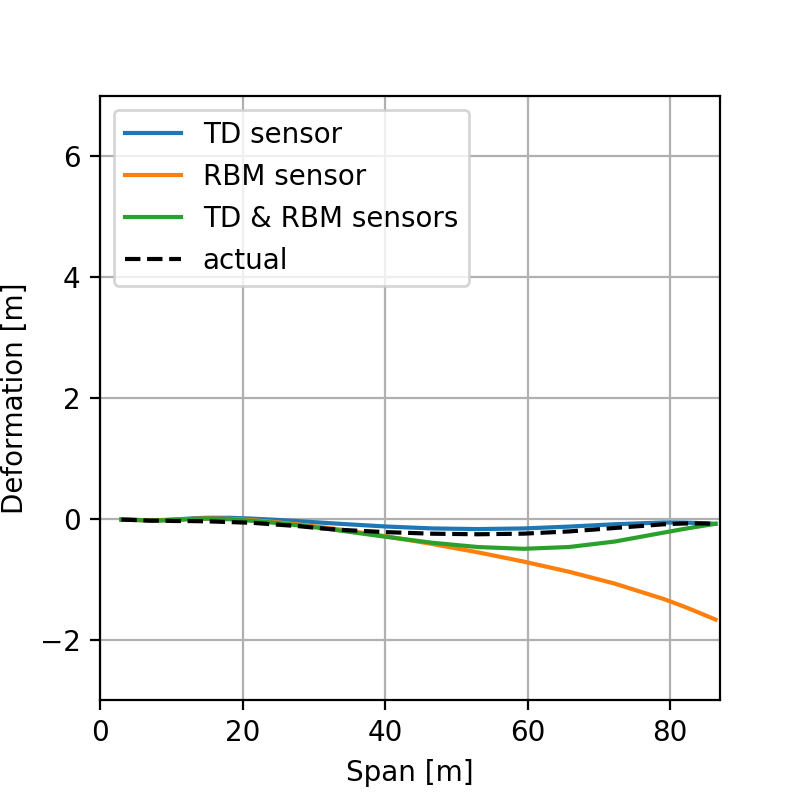
\includegraphics[width=1\textwidth]{Figures/TD_RBM_BladeDeformationEstimation.png}
    \caption{\small a}
	\label{#3}
    \end{subfigure}
    \begin{subfigure}[b]{0.4\textwidth}
    
    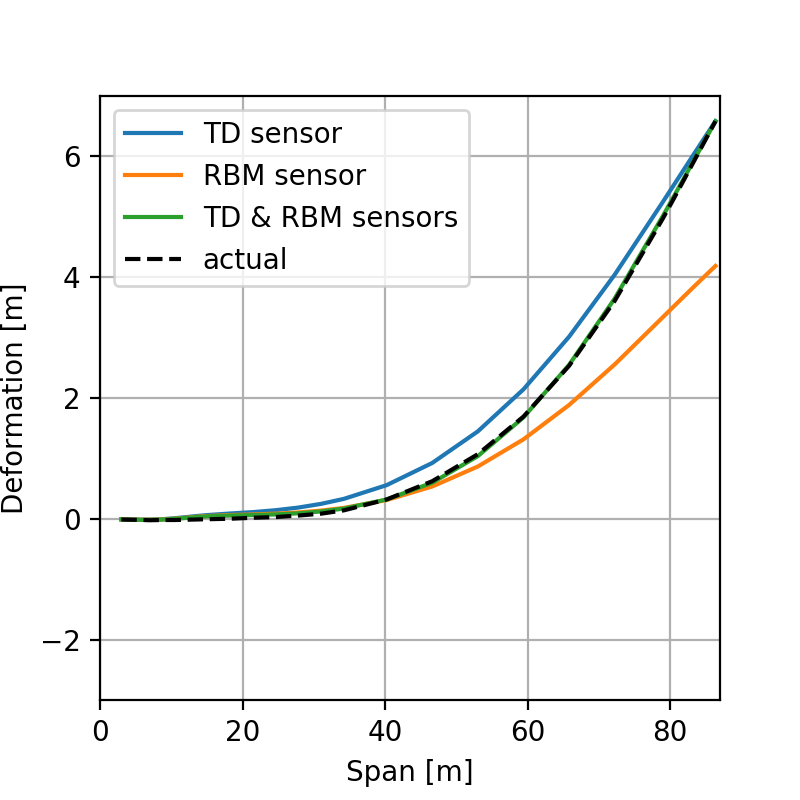
\includegraphics[width=1\textwidth]{TD_BladeDeformationEstimation.png}
    \caption{\small a}
	\label{#6}
    \end{subfigure}   
    \begin{subfigure}[b]{0.4\textwidth}
    
    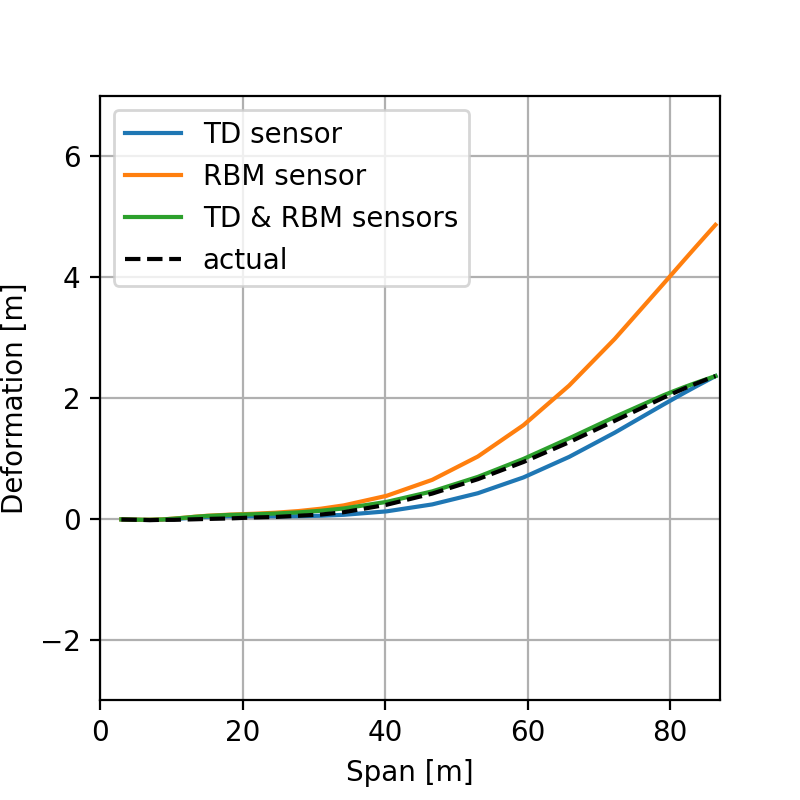
\includegraphics[width=1\textwidth]{RBM_BladeDeformationEstimation.png}
    \caption{\small a}
	\label{#6}
    \end{subfigure} 
    }
 	\setlength\fboxsep{1pt}
 	\setlength\fboxrule{0.5pt}
	\caption{\small a}
	\label{#8}
\end{figure}
\end{document}
